%% 
%% Copyright 2007-2020 Elsevier Ltd
%% 
%% This file is part of the 'Elsarticle Bundle'.
%% ---------------------------------------------
%% 
%% It may be distributed under the conditions of the LaTeX Project Public
%% License, either version 1.2 of this license or (at your option) any
%% later version.  The latest version of this license is in
%%    http://www.latex-project.org/lppl.txt
%% and version 1.2 or later is part of all distributions of LaTeX
%% version 1999/12/01 or later.
%% 
%% The list of all files belonging to the 'Elsarticle Bundle' is
%% given in the file `manifest.txt'.
%% 

%% Template article for Elsevier's document class `elsarticle'
%% with numbered style bibliographic references
%% SP 2008/03/01
%%
%% 
%%
%% $Id: elsarticle-template-num.tex 190 2020-11-23 11:12:32Z rishi $
%%
%%
\documentclass[preprint,12pt]{elsarticle}

%% Use the option review to obtain double line spacing
%% \documentclass[authoryear,preprint,review,12pt]{elsarticle}

%% Use the options 1p,twocolumn; 3p; 3p,twocolumn; 5p; or 5p,twocolumn
%% for a journal layout:
%% \documentclass[final,1p,times]{elsarticle}
%% \documentclass[final,1p,times,twocolumn]{elsarticle}
%% \documentclass[final,3p,times]{elsarticle}
%% \documentclass[final,3p,times,twocolumn]{elsarticle}
%% \documentclass[final,5p,times]{elsarticle}
%% \documentclass[final,5p,times,twocolumn]{elsarticle}

%% For including figures, graphicx.sty has been loaded in
%% elsarticle.cls. If you prefer to use the old commands
%% please give \usepackage{epsfig}

%% The amssymb package provides various useful mathematical symbols
\usepackage{amssymb}
%% The amsthm package provides extended theorem environments
%% \usepackage{amsthm}

%% The lineno packages adds line numbers. Start line numbering with
%% \begin{linenumbers}, end it with \end{linenumbers}. Or switch it on
%% for the whole article with \linenumbers.
%% \usepackage{lineno}
\usepackage{caption}
\usepackage{subcaption}
\usepackage[table]{xcolor}
\biboptions{sort&compress,super}

\usepackage{tabularray}
\newcommand{\beginsupplement}{%
        \setcounter{table}{0}
        \renewcommand{\thetable}{S\arabic{table}}%
        \setcounter{figure}{0}
        \renewcommand{\thefigure}{S\arabic{figure}}%
     }

\journal{Lancet Public Health}

\begin{document}

\begin{frontmatter}

%% Title, authors and addresses

%% use the tnoteref command within \title for footnotes;
%% use the tnotetext command for theassociated footnote;
%% use the fnref command within \author or \address for footnotes;
%% use the fntext command for theassociated footnote;
%% use the corref command within \author for corresponding author footnotes;
%% use the cortext command for theassociated footnote;
%% use the ead command for the email address,
%% and the form \ead[url] for the home page:
%% \title{Title\tnoteref{label1}}
%% \tnotetext[label1]{}
%% \author{Name\corref{cor1}\fnref{label2}}
%% \ead{email address}
%% \ead[url]{home page}
%% \fntext[label2]{}
%% \cortext[cor1]{}
%% \affiliation{organization={},
%%             addressline={},
%%             city={},
%%             postcode={},
%%             state={},
%%             country={}}
%% \fntext[label3]{}

\title{How city design contributes to changes in road transport mode choice and health risks during a crisis: a global observational study}

%% use optional labels to link authors explicitly to addresses:
%% \author[label1,label2]{}
%% \affiliation[label1]{organization={},
%%             addressline={},
%%             city={},
%%             postcode={},
%%             state={},
%%             country={}}
%%
%% \affiliation[label2]{organization={},
%%             addressline={},
%%             city={},
%%             postcode={},
%%             state={},
%%             country={}}

\author[melb]{Kerry~A.~Nice\corref{cor1}}
\author[melb]{Jason Thompson}
\author[melb]{Haifeng Zhao}
\author[melb]{Sachith Seneviratne}
\author[RMII]{Belen Zapata-Diomedi}
\author[Belfast]{Leandro Garcia}
\author[Belfast]{Ruth Hunter}
\author[wash]{Rodrigo Siqueira Reis}
\author[uill]{Pedro C. Hallal}
\author[melb,eng]{Mark Stevenson}
\author[melb]{et al.}

\cortext[cor1]{Principal corresponding author}
\ead{kerry.nice@unimelb.edu.au}
\address[melb]{Transport, Health, and Urban Systems Research Lab, Faculty of Architecture, Building, and Planning, University of Melbourne, VIC, Australia.}
\address[RMII]{Healthy Liveable Cities Lab, Centre for Urban Research, RMIT University, Melbourne, Australia.}
\address[Belfast]{Centre for Public Health, Queen’s University Belfast, Institute of Clinical Sciences B, Belfast, Northern Ireland, UK.}
\address[wash]{Washington University, St. Louis, Missouri, US.}
\address[eng]{Melbourne School of Engineering; and Melbourne School of Population and Global Health, University of Melbourne, VIC, Australia.}
\address[uill]{Department of Kinesiology and Community Health, University of Illinois Urbana-Champaign}

%\affiliation{organization={},%Department and Organization
%            addressline={}, 
%            city={},
%            postcode={}, 
%            state={},
%            country={}}

%\begin{abstract}
%% Text of abstract

%\end{abstract}

%%Graphical abstract
%\begin{graphicalabstract}
%\includegraphics{grabs}
%\end{graphicalabstract}

%%Research highlights
%\begin{highlights}
%\item Research highlight 1
%\item Research highlight 2
%\end{highlights}

%\begin{keyword}
%% keywords here, in the form: keyword \sep keyword

%% PACS codes here, in the form: \PACS code \sep code

%% MSC codes here, in the form: \MSC code \sep code
%% or \MSC[2008] code \sep code (2000 is the default)

%\end{keyword}

\end{frontmatter}

%% \linenumbers

%% main text

\section*{Introduction}

City designs are highly influenced by the dominant transport modes present at the time of their development\cite{KNOWLES2020102607}. These designs reflect a current snapshot of a dynamic, iterative process \cite{Strano2012}, with variations seen between and within individual cities, and form a scaffold upon which citizens move and interact\cite{Thompson2020}. City designs therefore both afford and constrain transport mode choice and significantly influence mobility patterns, influencing lifestyles and exposure to health risks\cite{WHO2023}.

Over 2020 and 2021, the global spread of CoVID-19 was reported by governments to have caused 5.4 million deaths, although the true death toll has been estimated to be up to 14.9 million\cite{Taylor2022}. This global crisis prompted a range of responses from governments\cite{Hunter2023LPH} to contain the spread and reduce public health injuries, resulting in rapid changes in urban mobility rates impacting both pollution levels and public health. While many of the policy choices\cite{hale2021global} might have been similar across different countries and cities, such as restrictions on movement, closing non-essential retail, or work at home orders, the urban form of each individual city was highly influential in how those policies played out.

The design of cities can arise from strict top-down planning regimes\cite{mundigo1977city} or organically through bottom-up processes\cite{batty2017thinking}. While some city designs foster movement and patterns of interaction that reduce exposure to significant health risks including air pollution, physical inactivity and concomitant chronic diseases, others exacerbate such concerns\cite{Wijnands2022, Stevenson2016,wang2023flood, stanley2022managing}. Given that approximately 56 percent of the world's 8 billion population lives in cities -- with projections it will reach 68 percent by 2050\cite{WHO2023}  -- understanding the role of city design in mitigation and prevention adverse health outcomes is of paramount importance in efforts to reduce the global burden of disease. 

Ready access to large-scale, standardised data enables exploration of the role that city design plays in mitigating or exacerbating health risks. However, accessing the necessary data is a challenge given the majority of globally available data sources at the level of the city are held in the Global North, while the majority of the world's urban population lives in the Global South\cite{Smit2021}.

There is evidence underlying  how varied public health risks such as overweight, obesity, mental illness, respiratory disease, and other health issues entwined with inequality and social disadvantage are entrenched in the fabric of city designs, whether planned or otherwise\cite{borrell2013factors,xing2016impact,yuchi2020road}. Not all cities nor parts of cities are on equal footing when faced with public health threats and hazards, with some citizens -- usually the most disadvantaged -- at greater risk of risk exposure and ill-health\cite{KRISHNA2021102046}. For example, social inequalities brought about through road and highway construction\cite{carpenter2010poverty,archer2020white} and the burden of disease attributable to road transport-related air pollution disproportionately affect poorer communities who live close to major roadways, children and the elderly. To illustrate, air pollution-related deaths peak among babies in the early (0-6 days) and late (7-27 days) neonatal groups, reflecting the role of particulate matter in causing lower-respiratory infections in newborns. These deaths then peak again in older age groups, as air pollution contributes to lower-respiratory infections as well as noncommunicable diseases that develop over time, such as ischaemic heart disease, stroke, chronic obstructive pulmonary disease (COPD), and lung cancer\cite{boogaard2022long}. 

Similarly, rates of road trauma are disproportionately high in cities and across locales within  cities where exposure to risk (i.e., through interaction with motor-vehicles) is greatest. Previous work\cite{Thompson2020} has identified nine main typologies of global urban form including sparsely or intensity developed areas, motor cities, high transit cities, cities with large blocks, irregular blocks, chequerboard arrangements, or cul de sacs. This work demonstrated that the per-capita burden of road transport injury for the poorest-performing global city types (motor cities dominated by motorised transport modes) is an estimated 2-times greater than the best performing city types, producing an estimated loss of nearly 9 million disability-adjusted life-years attributable to sub-optimal urban design per year\cite{Thompson2020}. Similarly, differences in road and intersection design within cities can produce considerable variation in risk exposure for residents within cities\cite{Wijnands_IntersectionDesign2021,MORRISON2019123}. Such elevated risk is in addition to that generated through auto-centric urban design that disproportionately forces car use and ownership upon already disadvantaged households\cite{currie2018alarming, CURL201861}. 

However, while roads and other transportation infrastructure are relatively static, risks are not. Risk exposure can shift dramatically in response to unfolding events and can be afforded or constrained by city design. For instance, cities with appropriate housing stock (e.g., large), industrial profile (e.g., service economy), demographic profile (e.g., nuclear families), and associated urban infrastructure (e.g., fast, widespread internet connection) may adapt readily to population-wide stay-in place policies triggered by biological or natural hazards\cite{hale2021global}. However, these population-wide policies can place long-term economic burden on people who remain in manual work or in roles that cannot be performed remotely\cite{CraigWFH,Vyas2021}. Such inequalities can heighten disadvantage for already vulnerable and high-risk communities\cite{martin2020fighting} which may in-turn foster resentment and broad-scale resistance toward observance of public health interventions\cite{de2016sustainability}. When high-risk groups reject public health guidance, risk to the general population is then elevated, especially in relation to communicable disease\cite{koopman2005control}.

Cities are complex systems\cite{DiezRoux2015}, and interventions are unlikely to be felt equally across all levels of society. Solutions to crises or problems at hand are likely to set in motion a chain of secondary effects whose outcomes may be either uncertain or even unknown at the outset\cite{Sterman2006}. When urban planning regimes and city designs meet mass public health challenges that impact populations and unfold over varying time-scales\cite{casti2012x}, they pose significant planning, management, and communication challenges for policymakers\cite{thompson2022modelling,thompson2022framework}. Hence, public health interventions demand a nuanced understanding of both long-term and short-term  outcomes, secondary effects, and the likely time-frames within which they remain effective, accepted and/or justified in the context of the cities, populations, and political economies in which they are enacted\cite{dawson2016snakes, oliu2021sars}.

%\textbf{Objectives}

The objective of this paper is to describe how city designs influenced changes to travel patterns and mode share during the first year of the CoVID-19 pandemic. We set out to evaluate the changes in transport-related pollution levels (namely, \(PM_{2.5}\) and \(NO_{2}\)) and exposure to injury risk associated with transport use across 679 cities, worldwide. We aim to demonstrate how estimated disease risk estimates across all-cause mortality, cardiovascular disease, respiratory disease, road injuries, and infectious disease are associated with differences in urban design. 

We identify how different city designs both afford and/or constrain the ability of cities and their populations to adapt to and recover from crises such as the CoVID-19 pandemic. We extend this to identify which city designs demonstrate greater resilience against immediate and long-term global public health threats and discuss the implications of our findings for future public health challenges. This leads to our main research question: which city designs demonstrate the greatest resilience to both acute and chronic health challenges?


%\textbf{Main research question}

% Which city designs demonstrate the greatest resilience to both acute and chronic health challenges?


% \section*{Research in context}

% \textbf{Evidence before this study} 
% A paragraph about what existed before.

% \textbf{Added value of this study} 
% A paragraph about what the study provides.

% \textbf{Implications of all the available evidence} 
% A paragraph about the implications of the study.



\section*{Methods}

To explore patterns of resilience across 679 global cities, a number of datasets have been assembled and analysed. These include the network structures of urban transportation systems, historic and predicted pollution levels, mobility indicators across 2020, measures of individual disease transmission in 2020, and measures of structural dimensions of each individual city's design.

\subsection*{Data analysis}
\textbf{Characterisation of cities' design}
The first stage of this research was to create a representation of cities that accurately captured important features of city design related to mobility and public health. Analysing urban design centred around urban road networks has previously been undertaken in a number of ways, such as generating metrics of the `three Ds'\cite{Ewing2010}, density, diversity, and design (later updated to also include destination accessibility and distance to transit). Barthelemy (2011)\cite{Barthelemy2011} uses graph networks to derive measures of betweenness centrality, closeness, and connectedness between nodes of the network graphs. We utilise a graph neural network constructed utilising OpenStreetMap (OSM) road network data\cite{Boeing2017a}, in which roads (edges) are connected through nodes with annotated characteristics (i.e. road types, number of roads connecting through a node, etc.) attached to both, from 1632 global cities previously identified in Thompson et al. (2020)\cite{Thompson2020}. Due to lack of available pollution data in many cities, the final set of cities was reduced to 679 (Figures \ref{fig:africa}-\ref{fig:southhamerica}.) Graph neural networks work by forming high-dimensional hypotheses that can effectively represent the data input into them; in this case, road networks, public transit networks, and active transport networks (e.g., walking and cycling paths) derived from OSM data. In the context of understanding mobility patterns, the utilisation of OSM data offers significant advantages over sampled imagery data used in previous studies (e.g.\cite{Thompson2020,seneviratne2021self}) due to OSM data's high density and its capacity to represent features of an entire city, rather than relying upon sampled data from locations across cities. Furthermore, in comparison to the use of imagery data, the analysed road networks of each city present a direct, rather than inferred data source. The coverage of cities analysed are shown in Figure \ref{fig:clusters}.


\begin{figure}
\centering
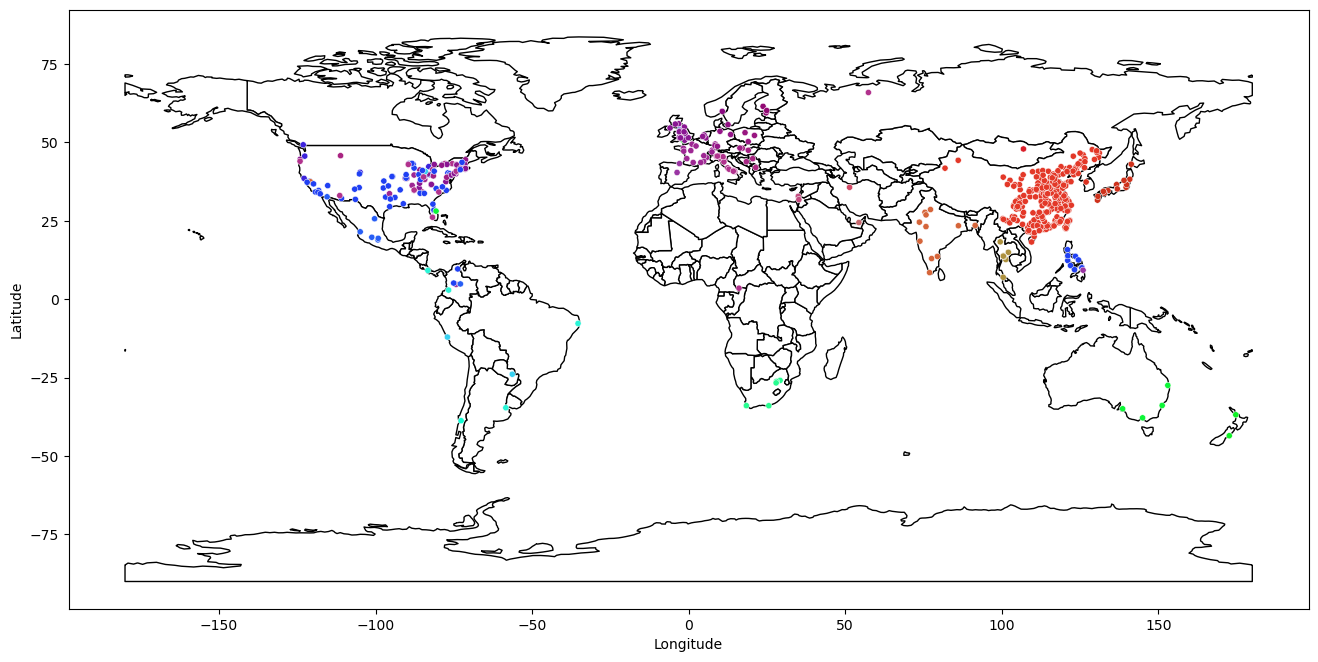
\includegraphics[trim={0 0 0 0},clip,scale=0.4]{Images/ByCountry_map_Zeigler.png}
\caption{\bf Location of the 679 cities used in this study.}
 \label{fig:clusters}
\end{figure}


The graph neural network was trained using self-supervised learning; a method proven to capture urban form comparably to supervised learning\cite{seneviratne2021self}. Importantly, this allows the graph neural network used here to represent the data without requiring a labelled output to the neural network, such as city names used in Thompson et al. (2020)\cite{Thompson2020}.

Masked Auto-encoding (MAE) was used as the training objective of the graph neural network. This objective has demonstrated effective performance in neural networks across various data modalities such as graphs\cite{hou2022graphmae}, images\cite{he2022masked}, graphs represented as images\cite{seneviratne2022self} and text\cite{devlin2018bert}. MAE trains the neural network by `masking' part of the input data, then tasking the model with predicting the masked (unknown) portion. Here, we masked both road (edge) features--such as length, start and end locations of roads--as well as node features such as latitude and longitude. The model then attempted to predict surrounding OSM sections from the remainder of the available sample. 

The results of this analysis were then converted to a t-SNE\cite{scikit-learn} graph which organised the average value of each city's OSM sample in a 2-dimensional plane where the distance between cities on the graph represented their similarities across urban characteristics (see Figure \ref{fig:tSNE}).

City-level pollution data (described in the next section) was employed to validate the representation learned by the neural network. For each city, the neural network could predict whether pollution levels rose or fell compared to the previous year with an accuracy of 97\%. This result underscores the neural network's ability to not only capture the road network of the modelled cities, but also to approximate the relationship between the transport network and the behaviour of pollutants within the city.

Additional validation of the neural network comes from Figure \ref{fig:Dimensions}, which plots the t-SNE representation against understood dimensions of urban design measured against city block size, block regularity (as measured by a summation of excess pixels for each block that do not fit in regular bounding boxes), and block number as well as percentage of road and transit networks observed in each city from prior studies\cite{Thompson2020,Nice2019b}. Combined with Figure \ref{fig:clusters} and Figure \ref{fig:tSNE}, Figure \ref{fig:Dimensions} demonstrates that the urban morphology for analysed cities follows gradual changes across dimensions. High-density, small-block size and relatively regular cities are depicted on the upper-left of the chart (e.g., in areas A1/A2 and B1/B2), whereas sparse, large-block cities with little public transit infrastructure as a proportion of the transport network cluster together in the bottom right through areas G7 to H7. 

Figure \ref{fig:tSNE} also shows that cities from within countries and continents tend to cluster together. For example, Japanese cities cluster tightly together across areas A1 and B1, while European cities cluster together in and around areas A2 to B2. Asian cities across China, India and Vietnam extend in a regular pattern from grid references B3 through to H7 as their designs differed along dimensions of block size and road network density.

Of note are also clusters of Australasian, South American and North American cities found in areas A3 to A5 and B3 to B5. Urban designs in these areas tended to demonstrate regular, medium-sized blocks with medium to low levels of public transit. Cities in these locations were typically of a `Chequerboard' or `Motor City' types, designed to facilitate the egress of motor vehicles.

\begin{figure}
\centering
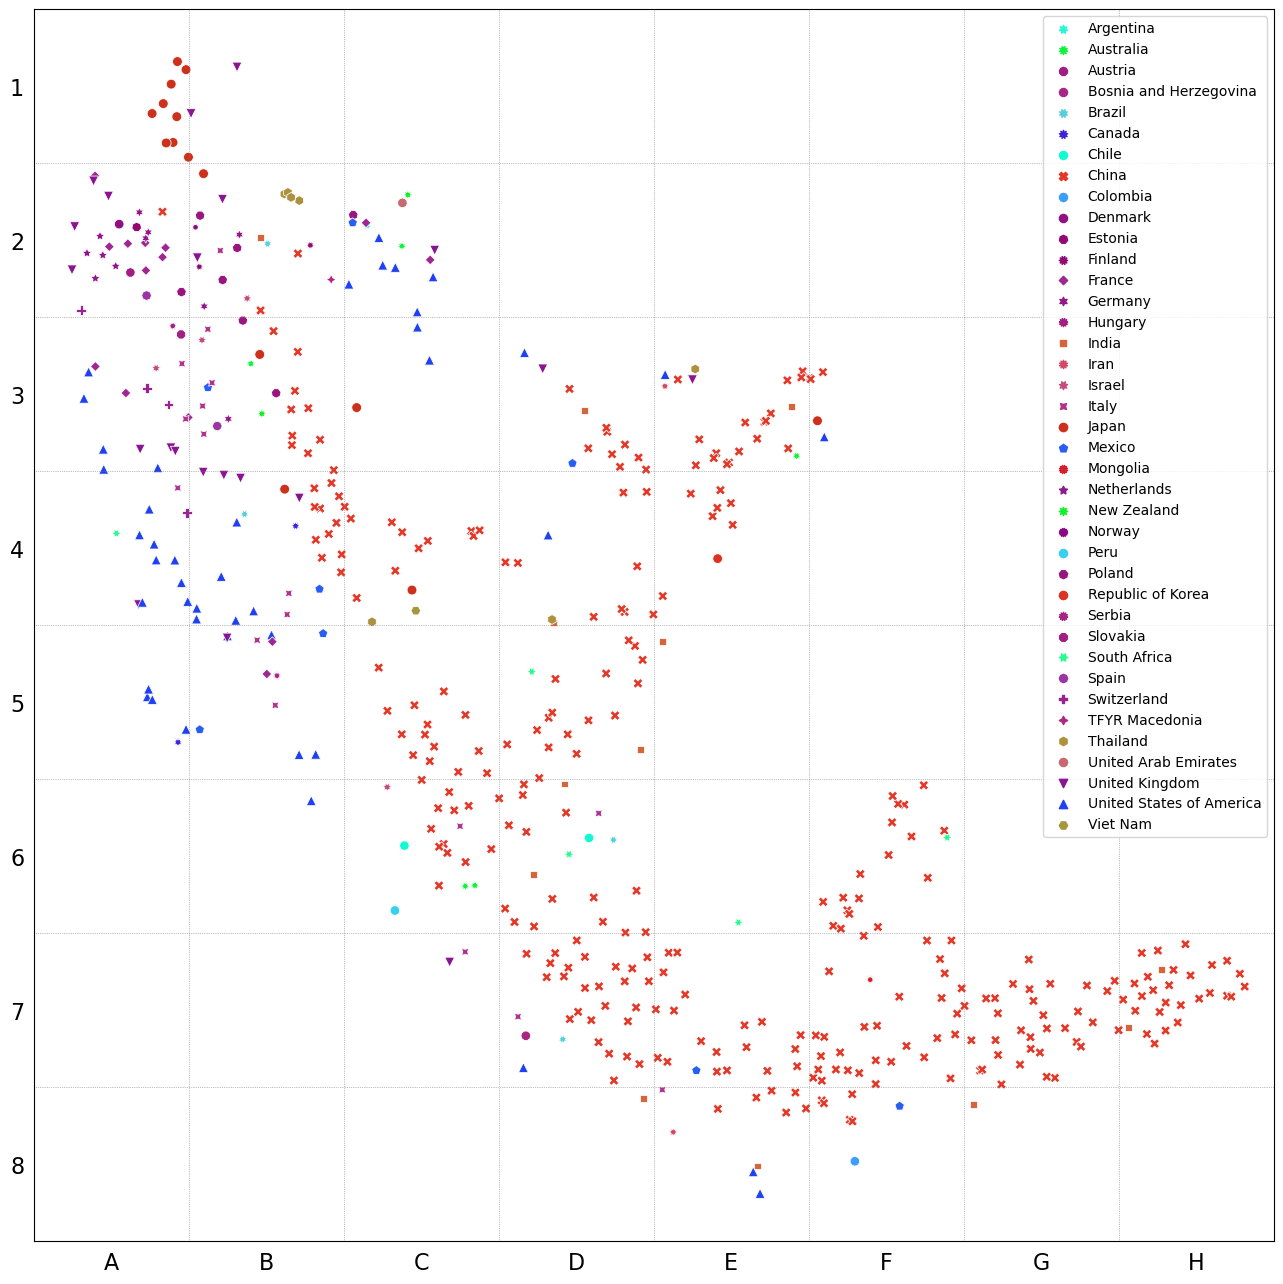
\includegraphics[trim={ 0 0 0 0 },clip,scale=0.45]{Images/ByCountry_latlong_Zeigler.png}%tSNE Country.png}
\caption{\bf t-SNE 2-dimensional representation of 679 global cities, organised by similarities across urban characteristics from OpenStreetMap network graphs. Colour scheme indicates geographic latitude/longitude location\cite{Jackle2017} of each of the cities. Grid references (i.e. A1) are used in the text to describe regions in the graph.}
 \label{fig:tSNE}
\end{figure}


%\begin{figure}
%\centering
%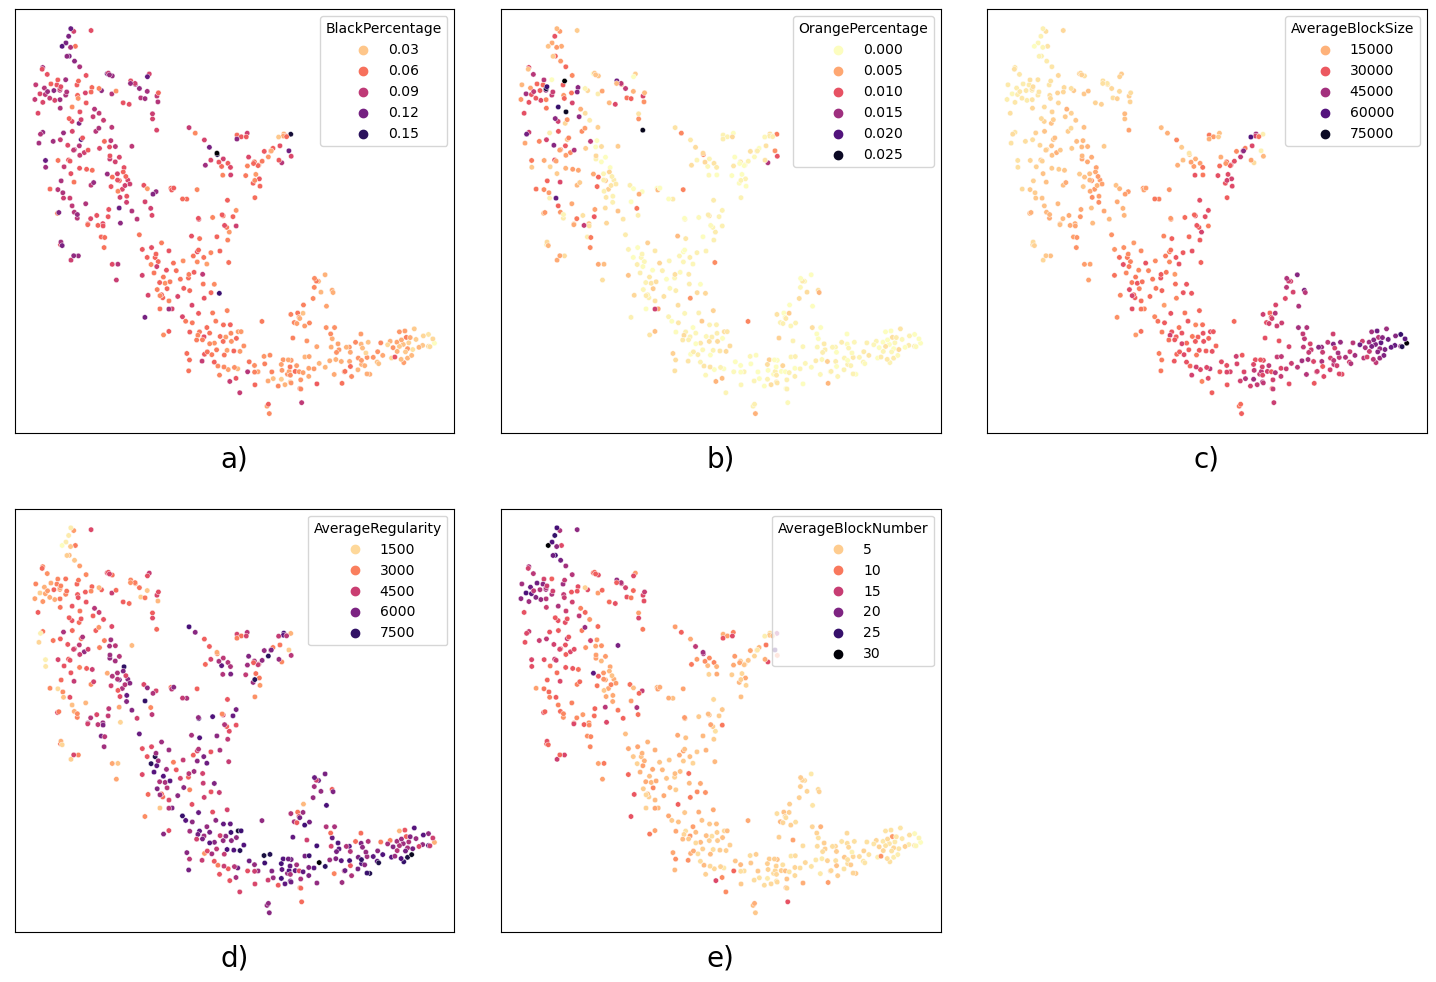
\includegraphics[trim={ 0 0 0 0 },clip,scale=0.35]{Images/City_Types_Dimension_axisoff.png}%City_Types_Dimension_chessboard.png%City Types Dimensions.png}

%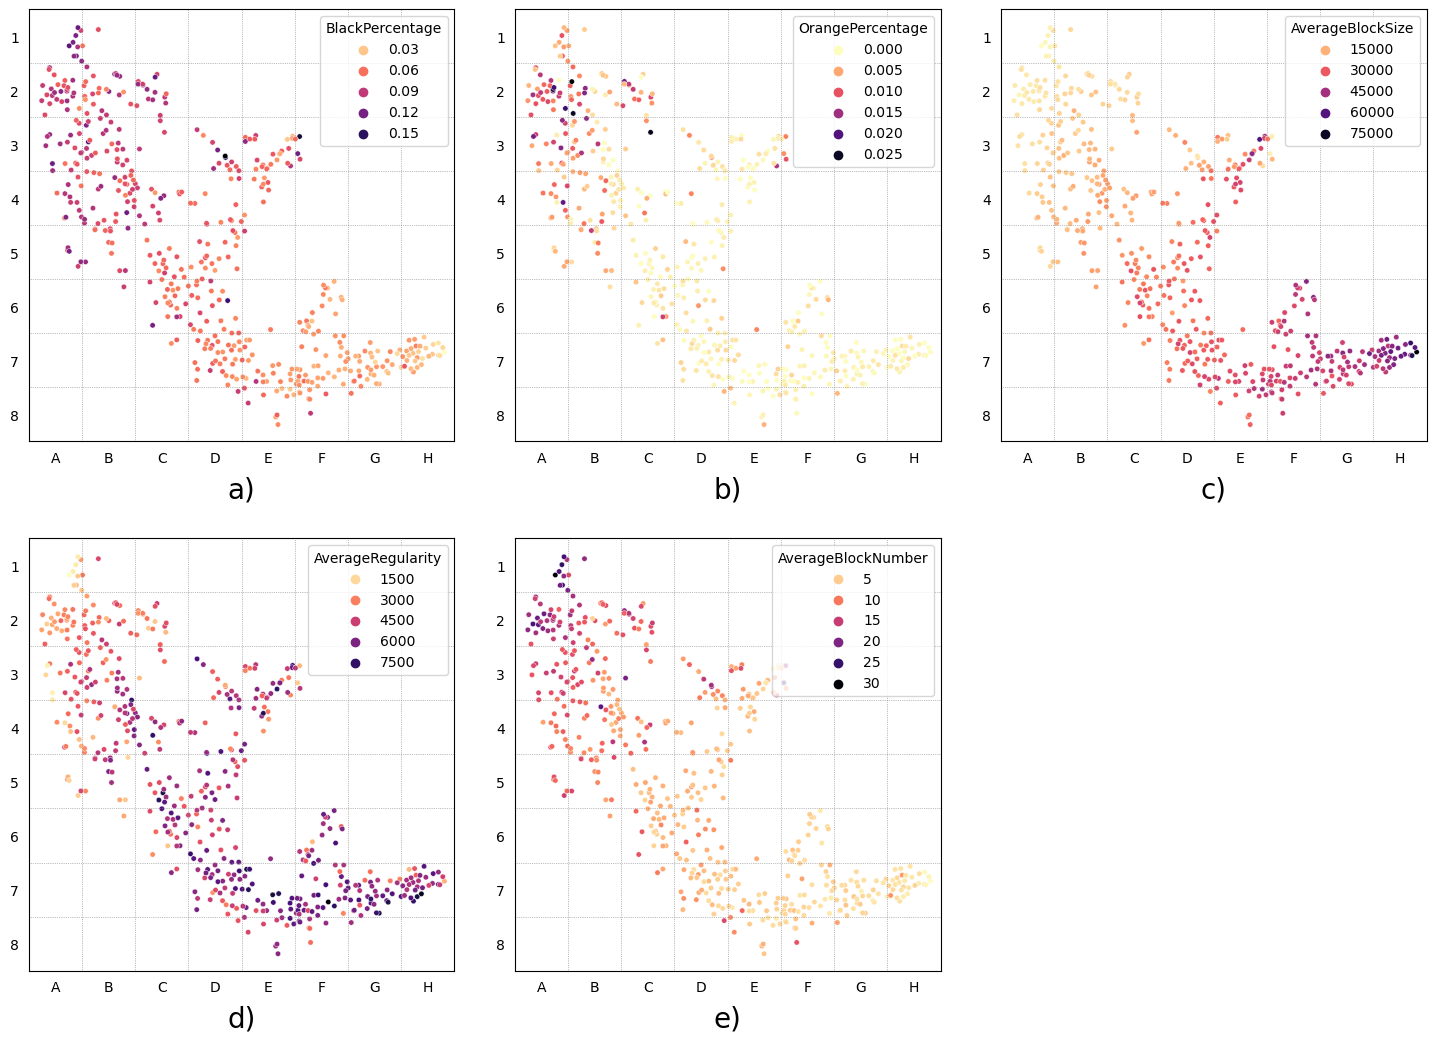
\includegraphics[trim={ 0 0 0 0 },clip,scale=0.35]{Images/City_Types_Dimension_chessboard.png}

%\caption{\bf Characteristics of 679 global cities (from Figure \ref{fig:tSNE}) showing percentages of a) black and b) orange pixels from sampled maps\cite{Thompson2020}, reflecting amounts of road space and public transport rail lines in each city. Panels c, d, and e) show average block sizes (m$^{2}$), a measure of city block regularity (lower values reflect increasing squareness), and a count of blocks per 400m area\cite{Nice2019b}. City locations and grid references are identical to those in Figure \ref{fig:tSNE}}
% \label{fig:Dimensions}
%\end{figure}


%\begin{figure}
%\centering
%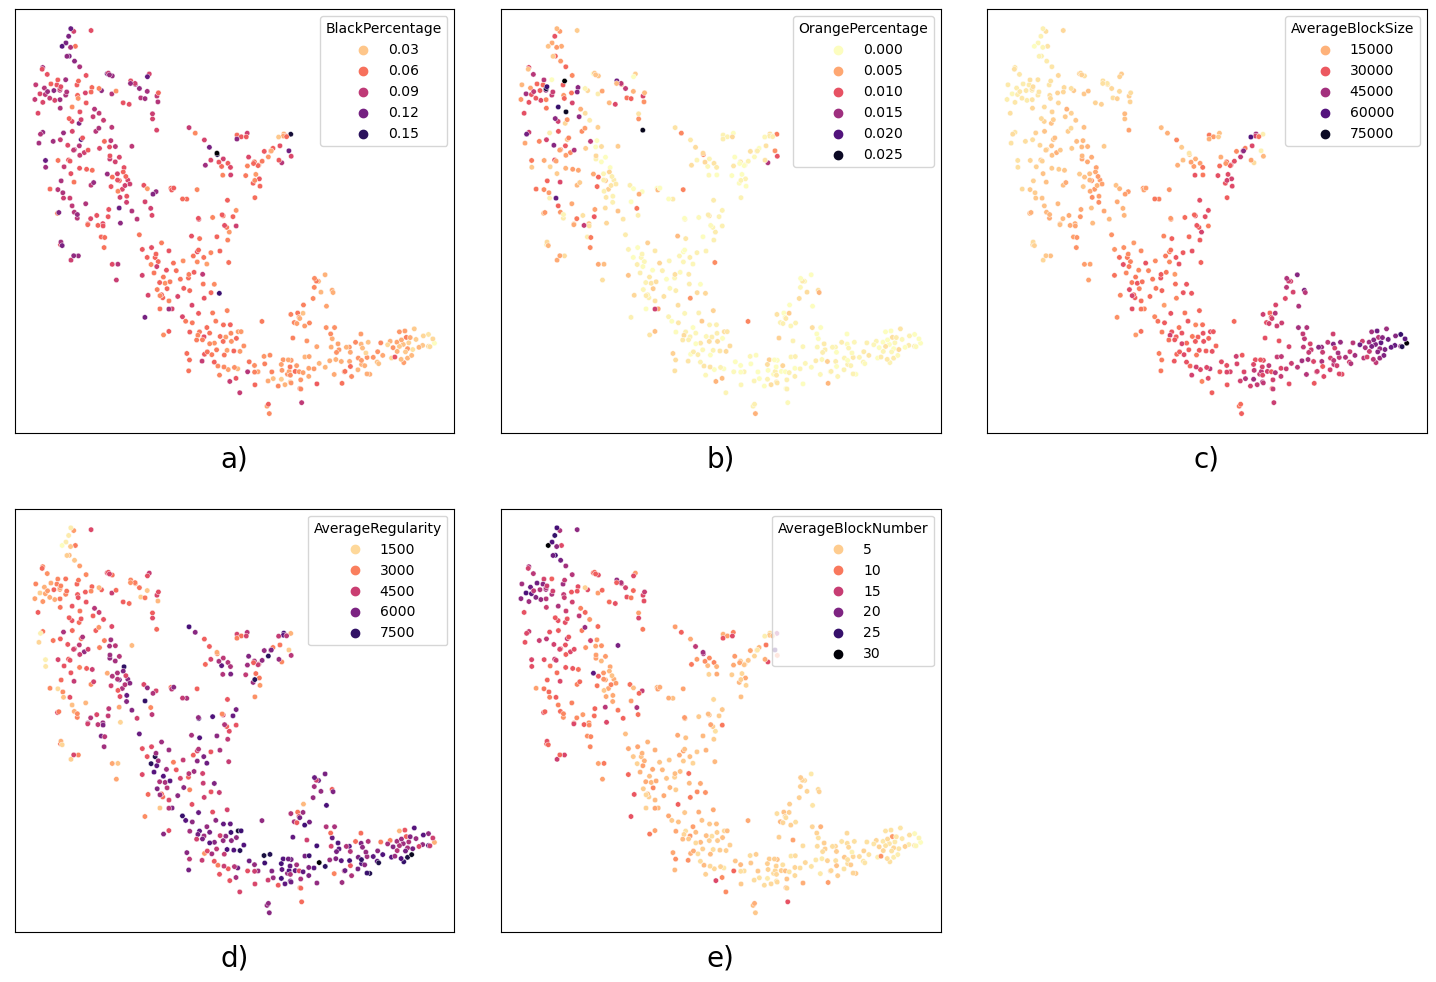
\includegraphics[trim={ 0 0 0 0 },clip,scale=0.35]{Images/City_Types_Dimension_axisoff.png}%City_Types_Dimension_chessboard.png%City Types Dimensions.png}
%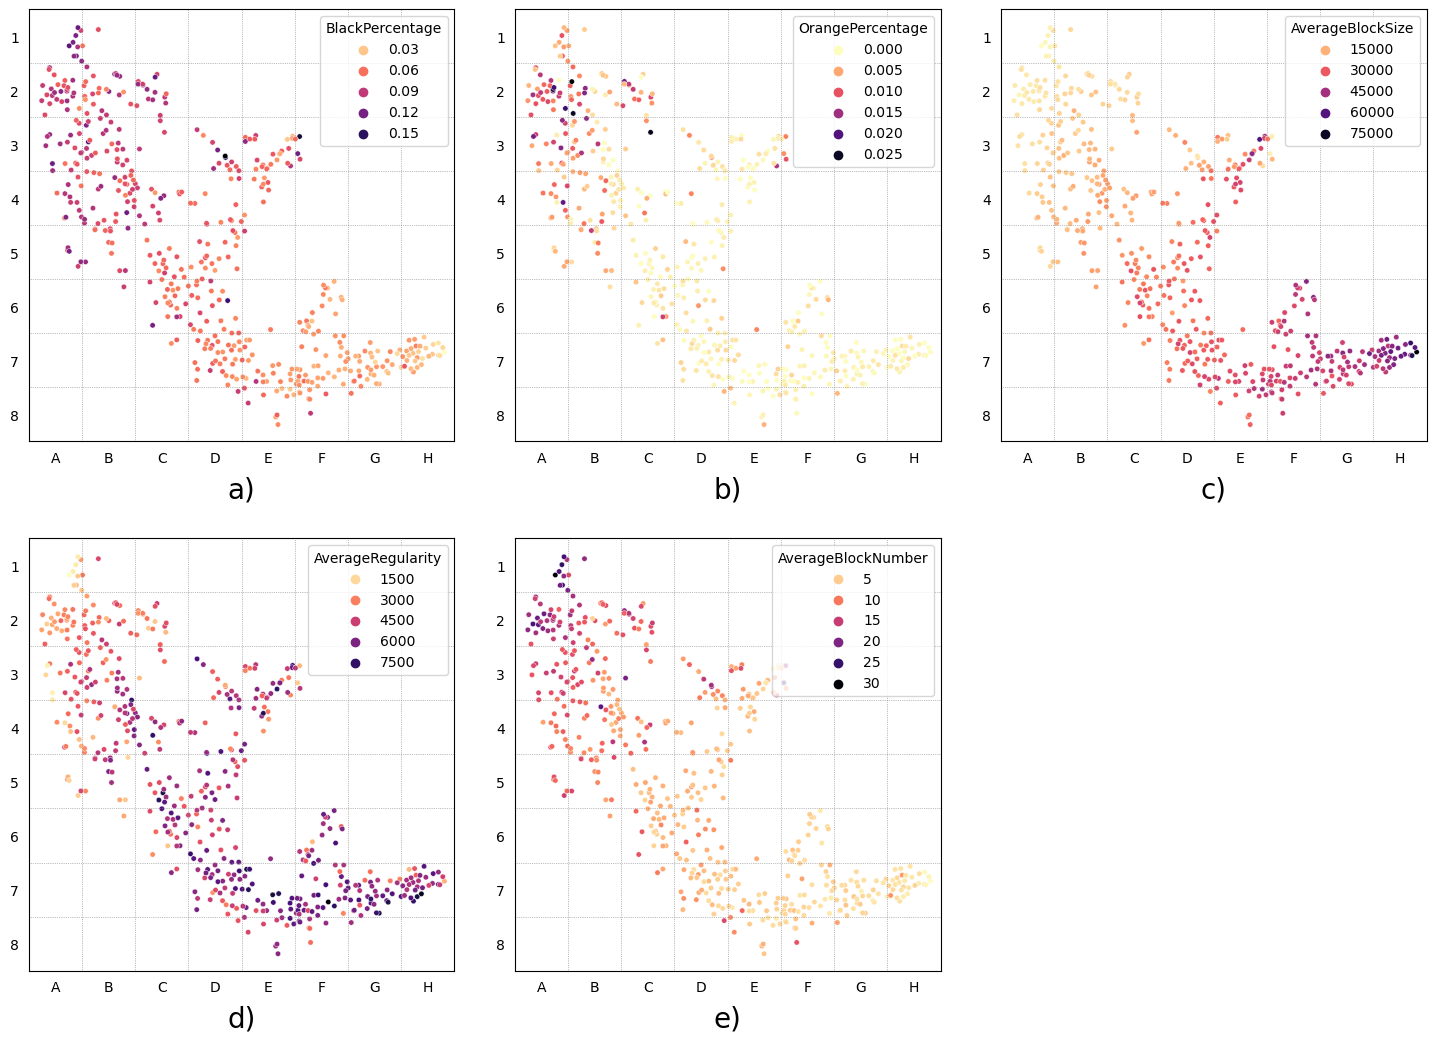
\includegraphics[trim={ 0 0 0 0 },clip,scale=0.35]{Images/City_Types_Dimension_chessboard.png}
%\caption{\bf Characteristics of 679 global cities (from Figure \ref{fig:tSNE}) showing percentages of a) black and b) orange pixels from sampled maps\cite{Thompson2020}, reflecting amounts of road space and public transport rail lines in each city. Panels c, d, and e) show average block sizes (m$^{2}$), a measure of city block regularity (lower values reflect increasing squareness), and a count of blocks per 400m area\cite{Nice2019b}. City locations and grid references are identical to those in Figure \ref{fig:tSNE}}
% \label{fig:Dimensions}
%\end{figure}


\begin{figure}
\centering
%black percentage A
\scriptsize{a)} 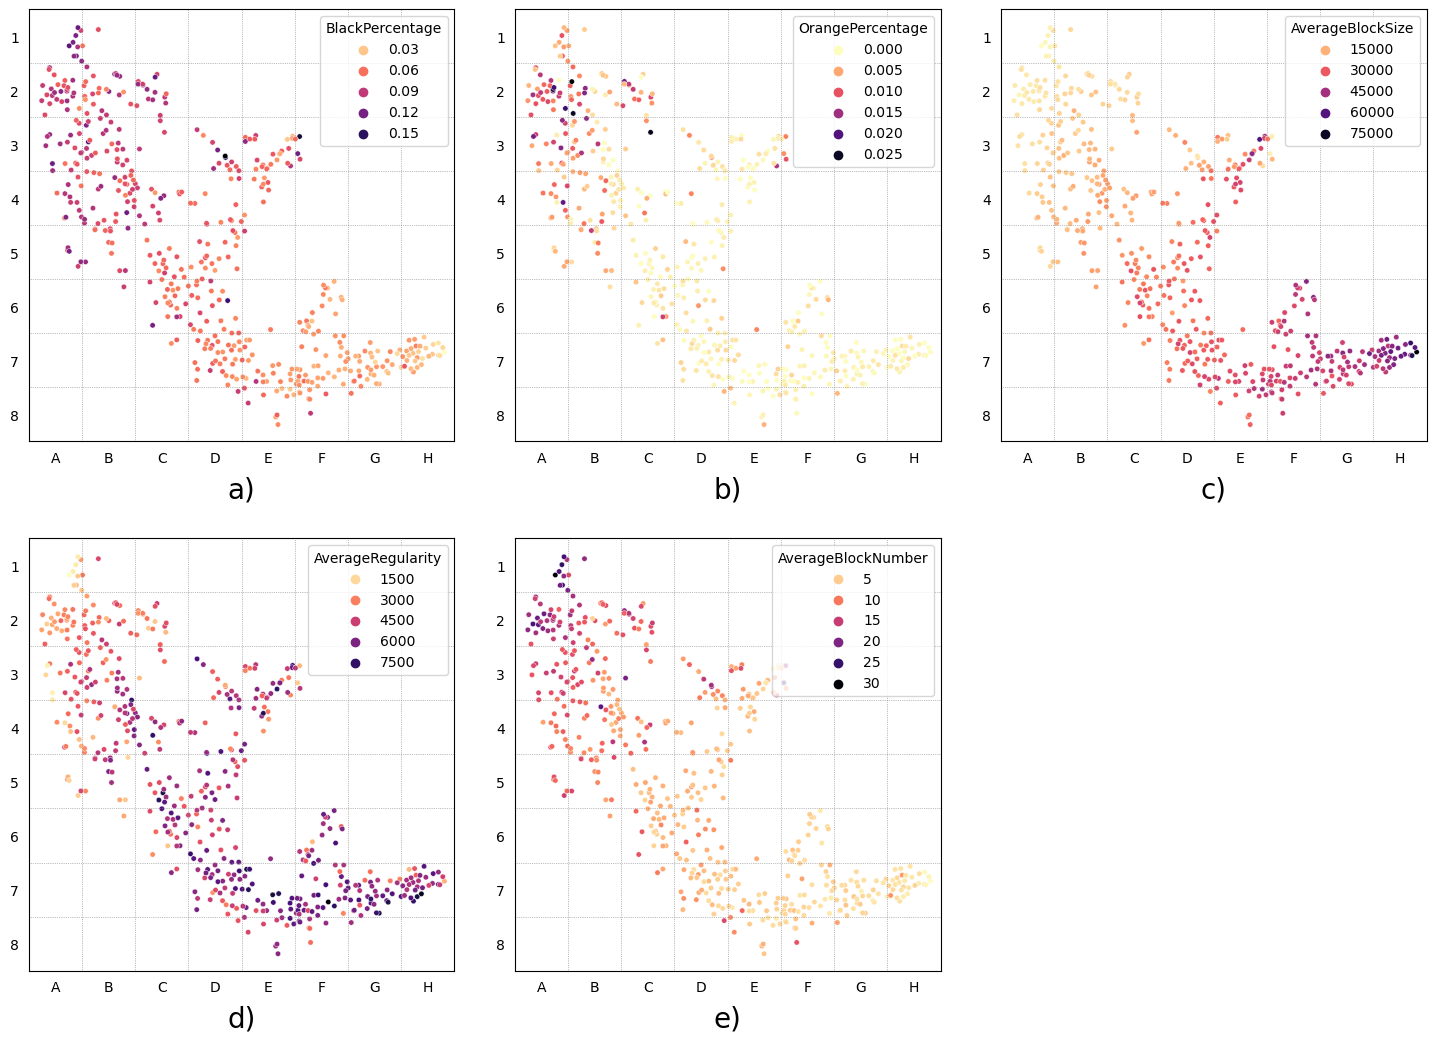
\includegraphics[trim={ 7 416 703 0 },clip,scale=0.40]{Images/City_Types_Dimension_chessboard.png}
% orange percentage B
\scriptsize{b)} 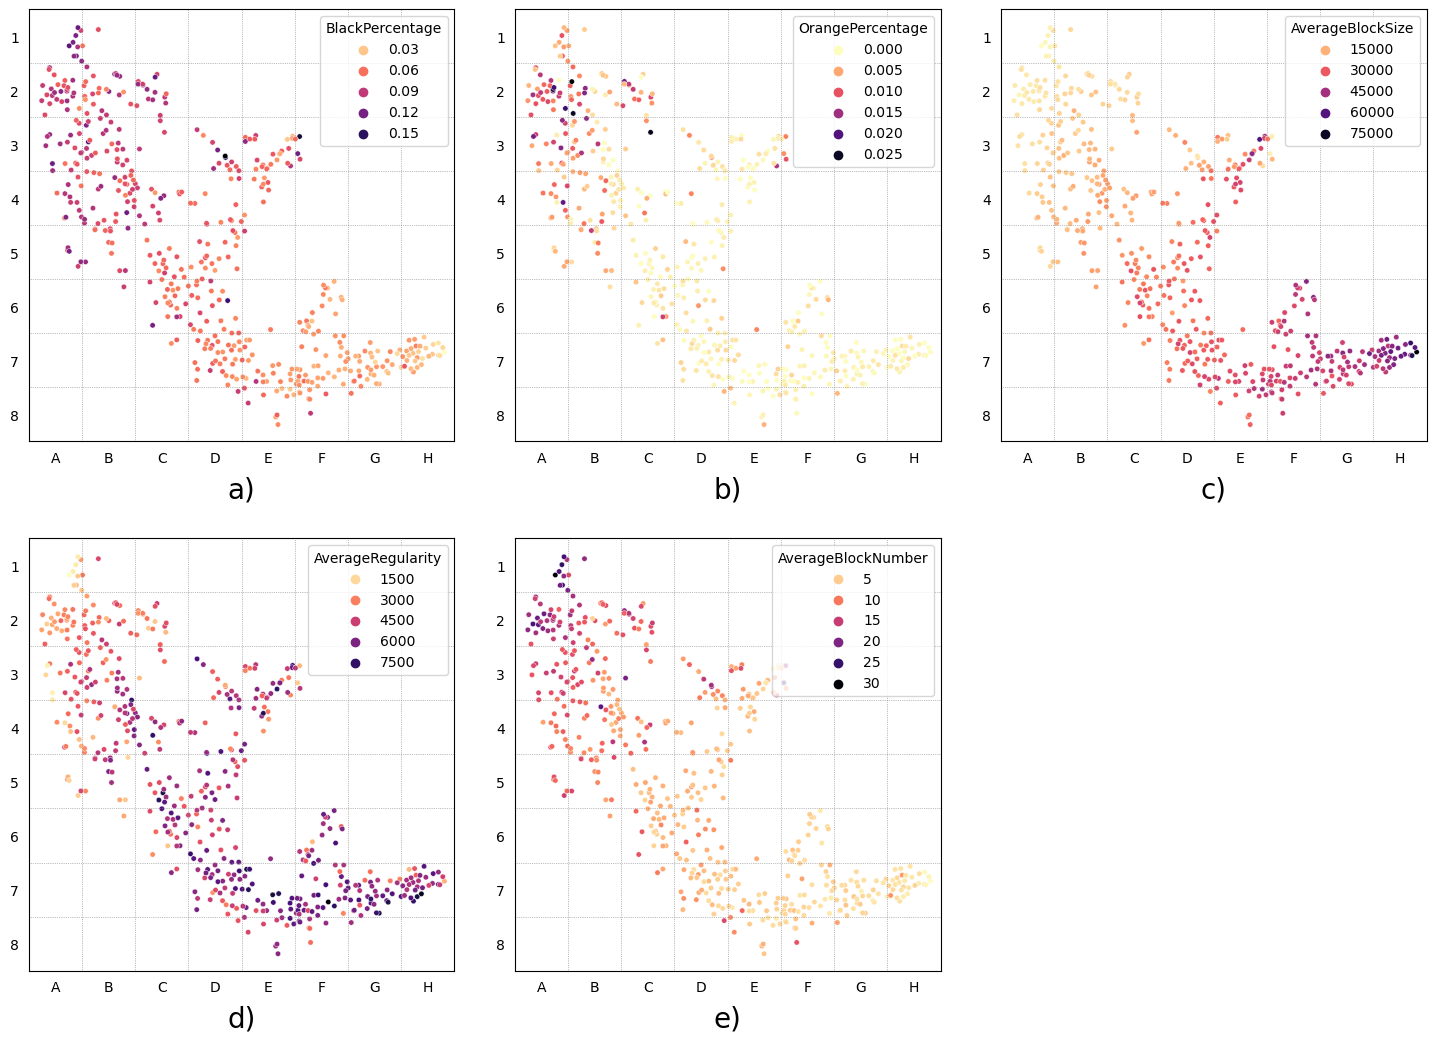
\includegraphics[trim={ 357 416 350 0 },clip,scale=0.40]{Images/City_Types_Dimension_chessboard.png}
% average block size C
\\ \scriptsize{c)} 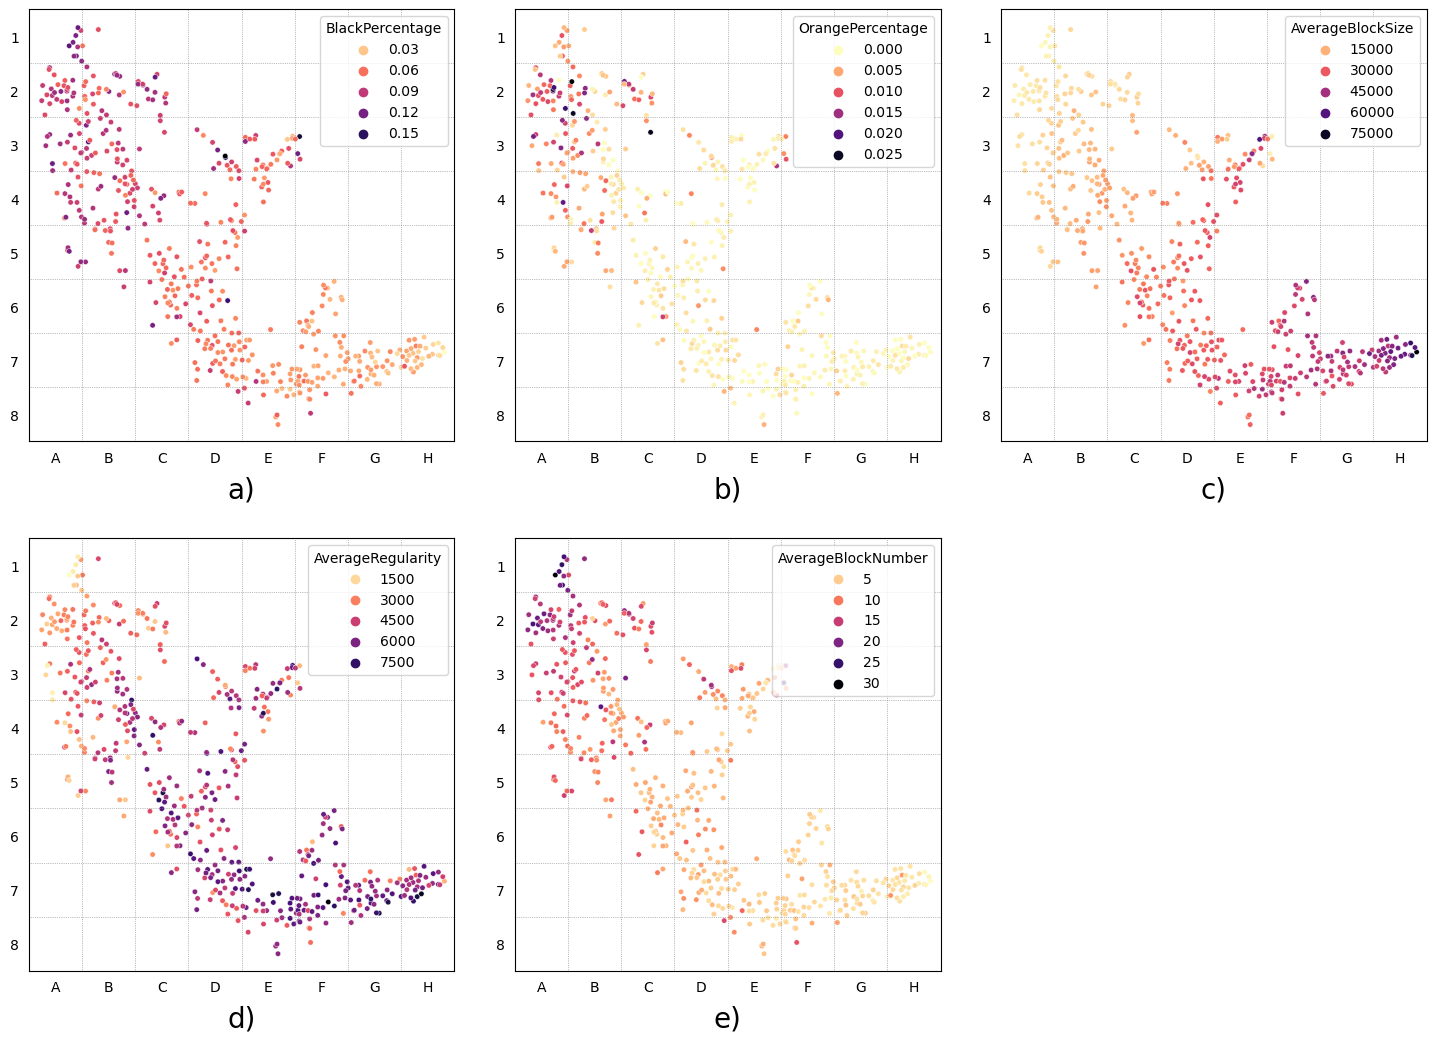
\includegraphics[trim={ 703 416 0 0 },clip,scale=0.40]{Images/City_Types_Dimension_chessboard.png}
% average regularity D
\scriptsize{d)} 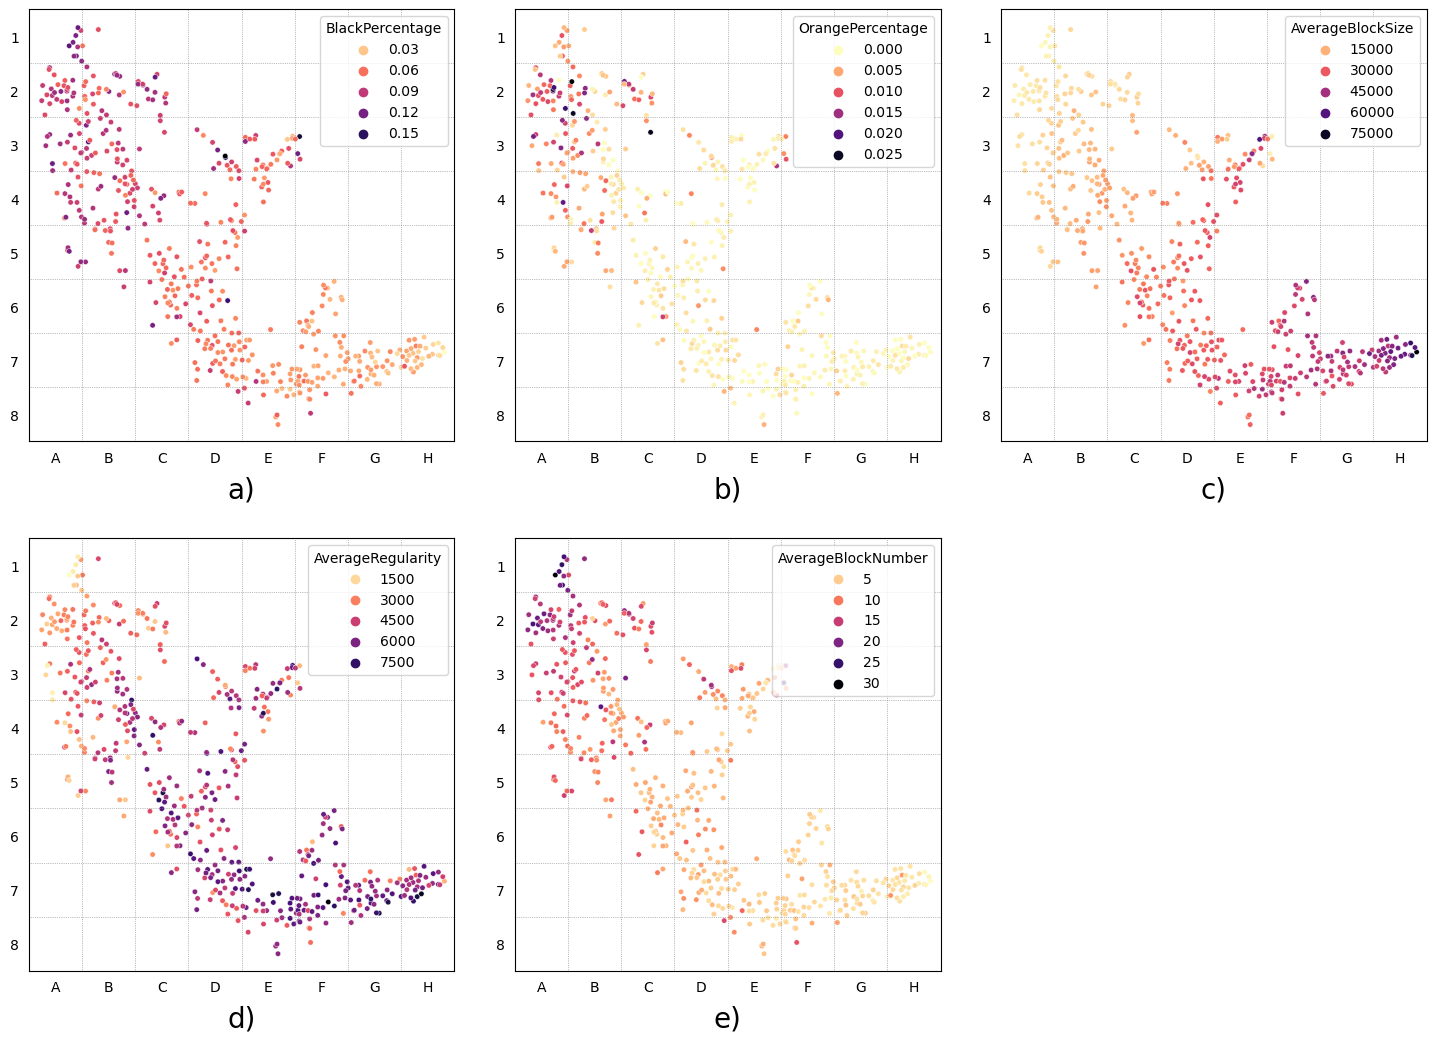
\includegraphics[trim={ 7 30 703 380 },clip,scale=0.40]{Images/City_Types_Dimension_chessboard.png}
% average blocks E
%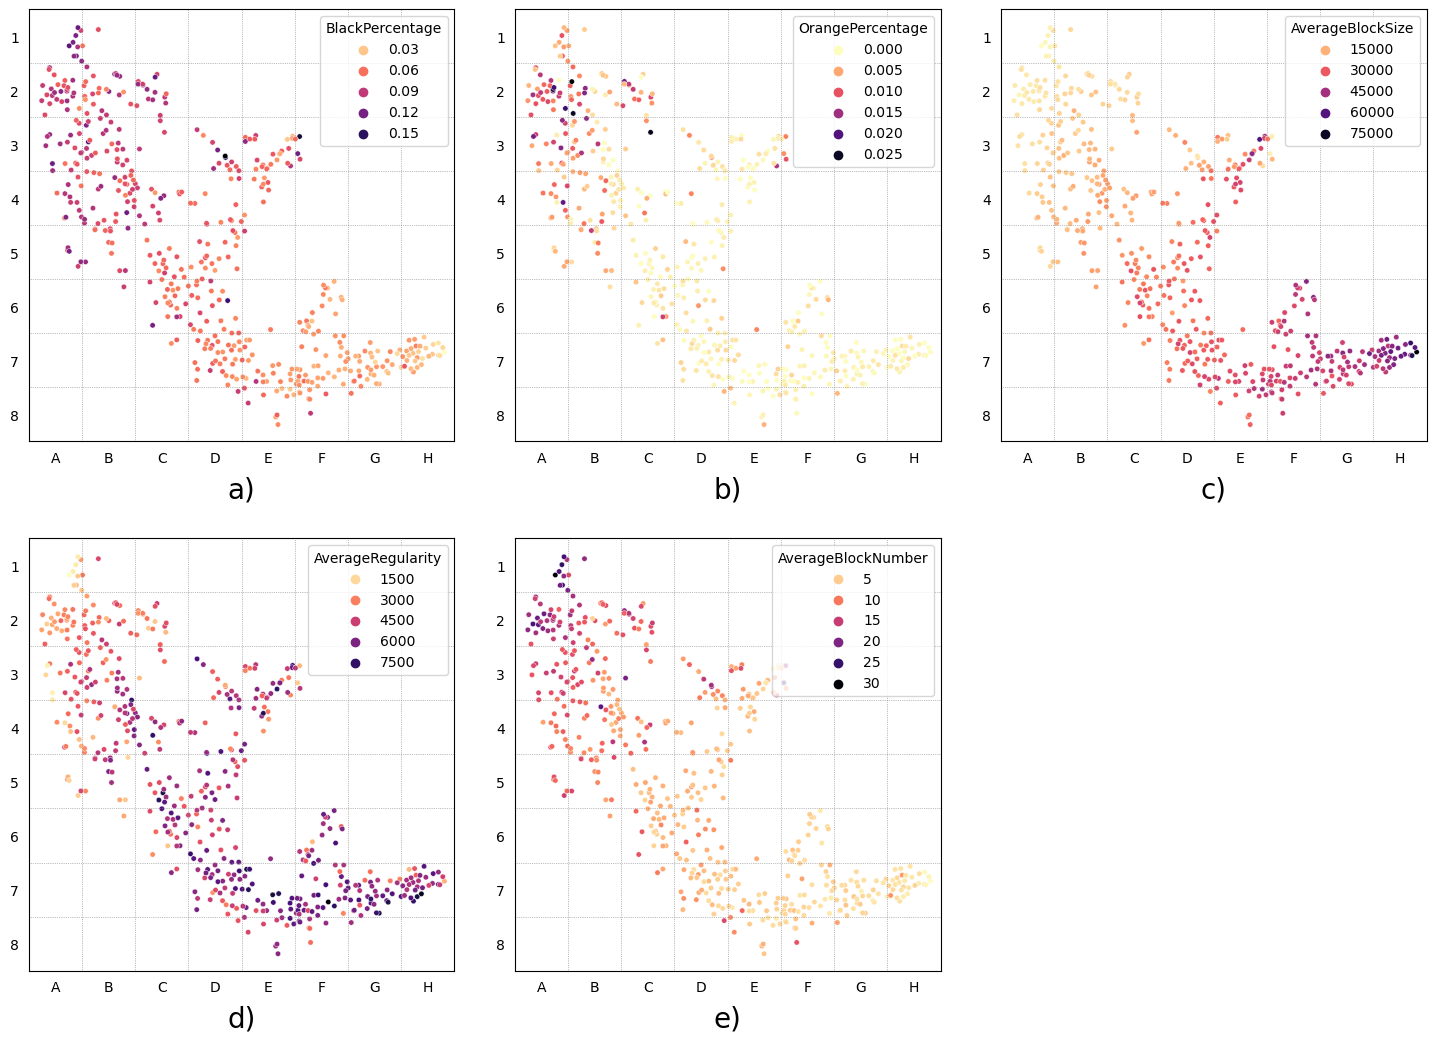
\includegraphics[trim={ 357 30 350 380 },clip,scale=0.35]{Images/City_Types_Dimension_chessboard.png}
\caption{\bf Characteristics of 679 global cities (from Figure \ref{fig:tSNE}) showing percentages\cite{Thompson2020} of a) black and b) orange pixels from sampled maps, reflecting amounts of road space and public transport rail lines in each city. Panels c) and d) show\cite{Nice2019b} average block sizes (m$^{2}$) and a measure of city block regularity (lower values reflect increasing squareness). City locations and grid references correspond to those in Figure \ref{fig:tSNE}}
 \label{fig:Dimensions}
\end{figure}




\subsection*{Data sources}\label{sec:datasources}


Wijnands et al. (2022)\cite{Wijnands2022} created pollutant and city specific XGBoost models for 679 cities, trained on weather and pollution observations over 2015-2019 and used these models to predict daily pollution levels of NO$_{2}$, PM$_{2.5}$, PM$_{10}$, and O$_{3}$ during 2020. Using 2020 observed values, anomalies were calculated in the absence of a pandemic. The original Thompson et al. (2020)\cite{Thompson2020} urban typology dataset consisted of the largest 1632 cities in the world. Of these, a subset of 679 cities were used (see Figure \ref{fig:clusters}), those that had pollution data available.

Apple\cite{Apple2020} and Google\cite{Google2020} provided mobility indexes in 2020. Apple's index calculates differences in map requests for modes of walking, driving, or public transit over a January 2020 baseline provided as a ratio. Google generated an index using phone-tracking-based changes in mobility across several types of locations, including retail and recreation, grocery stores and pharmacies, parks, transit stations, workplaces, and private residences. These daily indexes were linked to the 679 cities with available pollution data with changes representing percentage differences in attendance from a 5-week pre-pandemic baseline from January 3rd to February 6th, 2020\cite{owidcoronavirus}.

Google's CoVID-19 Open Data repository\cite{Google2022} provides data for daily CoVID-19 cases using a consistent set of region keys. Daily values were linked to the 679 cities when city case data was available, matching country-level to cities when city-level data was unavailable. This data was curated by Wahltinez et al. (2020) \citep{Wahltinez2020}, retrieved directly from the relevant authorities, like a country's ministry of health.

Associations between pollution data at the city level and estimated health risk impacts were made for NO2 across all-cause mortality, cardiovascular disease, and respiratory disease \cite{Huang19Pollution}. Similarly, changes in PM2.5 pollution levels were associated with estimated changes in health risk for all-cause mortality, ischaemic heart disease mortality, and Type 2 diabetes \cite{Xie257, Yu2020PM2.5}. Due to extreme pollution measurements in some locations, estimated changes in relative health risks from baseline were conservatively capped at 2x risk at the upper level. Estimates for all health outcomes were calculated for each city, and also aggregated to the continent and overall level for analysis. 


\begin{figure}
\centering
%\fbox{
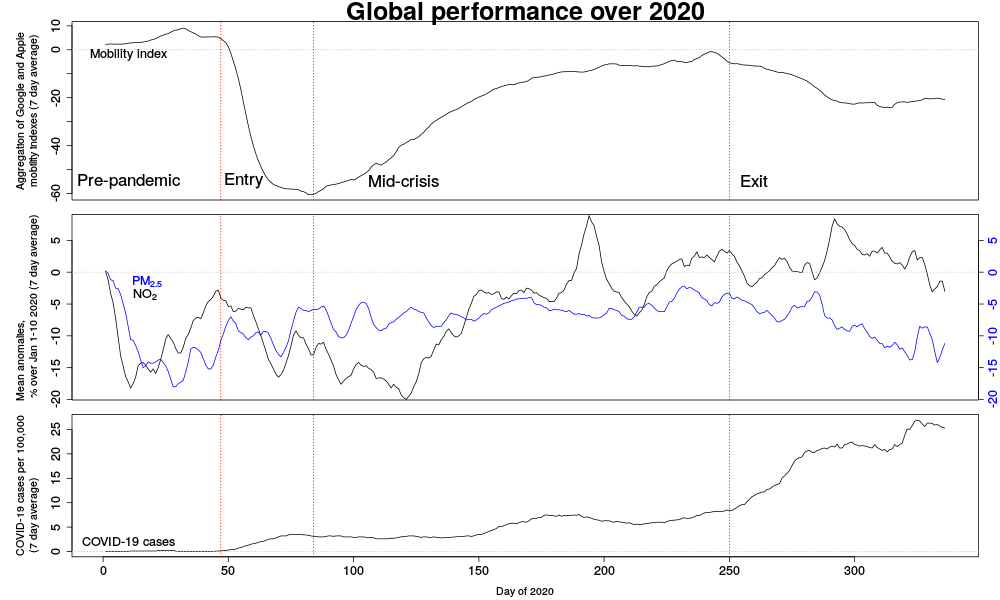
\includegraphics[trim={0 0 15 20},clip,scale=0.45]{Images/LancetPHOverall.png}
%}
\caption{\bf Overview of CoVID-19 crisis progression and stages across 679 global cities over 2020. Seven day rolling average aggregations of Google and Apple mobility indexes (top), seven day rolling averages of pollution percentage anomalies (PM$_{2.5}$ in blue and NO$_{2}$ in black) over January 1-10, 2020 baseline (middle), and seven day rolling average CoVID-19 cases per 100k (bottom).}
 \label{fig:stages}
\end{figure}

\section*{Results}

\begin{figure}
\centering
%\fbox{
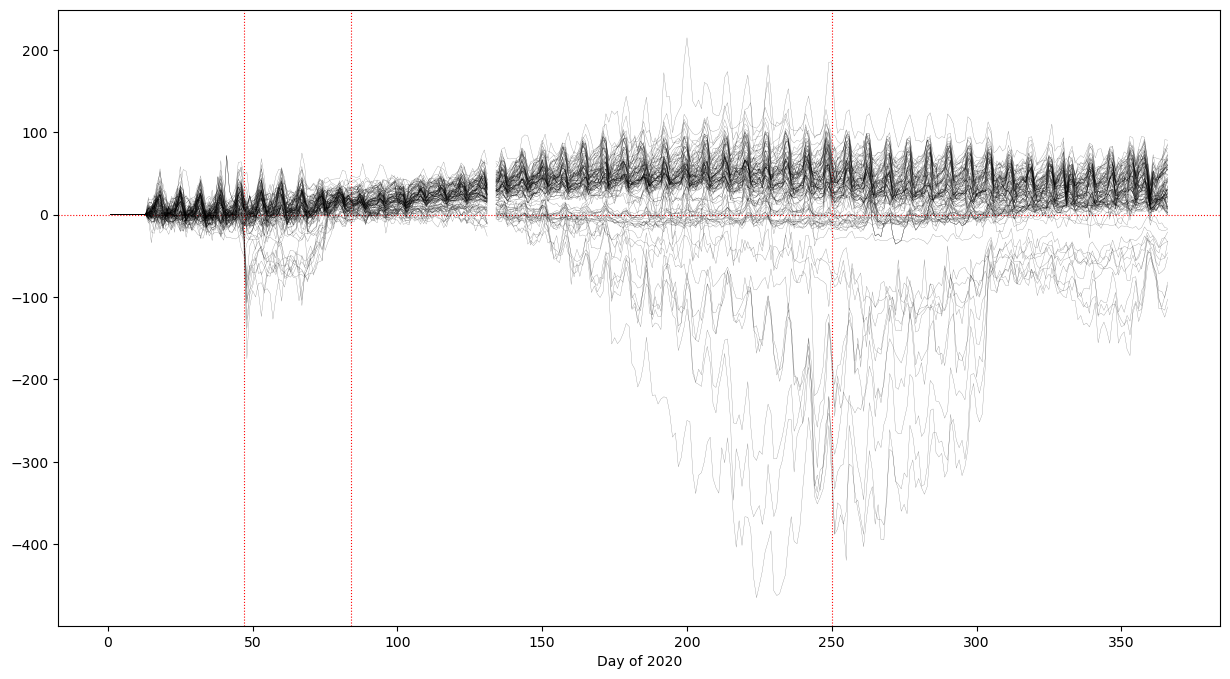
\includegraphics[trim={0 0 0 0},clip,scale=0.4]{Images/DrivingvsTransit.png}
%}
\caption{\bf An overview of observed modal shift from public transit to private motor vehicles observed during 2020 for all analysed cities highlighting an increased reliance on private vehicle use over public transit during the course of the CoVID-19 pandemic. Values \textgreater 0 indicate a proportional replacement of public transit trips to private vehicles for individual cities in comparison to pre-pandemic conditions.}  
 \label{fig:driv_trans}
\end{figure}


Figure \ref{fig:stages} shows average mobility (Panel 1), anomalies of NO$_{2}$ and PM$_{2.5}$ pollution levels (Panel 2), and total reported CoVID-19 cases (Panel 3) for all measured cities during 2020 across the `Pre-pandemic', `Entry', `Mid-Crisis', and `Recovery' phases of the CoVID-19 pandemic defined as between between days 0 and 46, 47 to 83, 84 to 250 and day 251+, respectively. Mobility measures are calculated as seven day rolling average aggregations of Google and Apple across the 679 cities for which data was available across both mobility and pollution. Pollution anomalies are calculated as percentage seven day rolling average differences over a January 1-10, 2020 baseline. CoVID-19 cases are calculated as a 7-day rolling average of cases per 100,000 population from Google (2022)\cite{Google2022}.

From Figure \ref{fig:stages} the impact on global mobility that resulted from the introduction of movement restrictions, including stay-at-home orders, implemented across global cities during the pandemic can be observed `Entry' phase\cite{hale2021global}. Although movement restrictions were designed as a public health measure to reduce person-to-person disease transmission, secondary effects related to reductions in global road trauma (refs) and significant reductions in mean transport-related NO$_{2}$ and PM$_{2.5}$ levels\cite{zhang2023impact}. Average mobility declined across cities, reaching a nadir at approximately 45 days post-pandemic onset. This period also coincided with a plateau in global CoVID-19 infection growth (Panel 3) not least because of the public observance of mobility restrictions as well as other non-pharmaceutical interventions implemented up to and including this time\cite{hale2021global}. 

The mean estimated reduction in global NO$_{2}$ and PM$_{2.5}$ levels across observed cities from the beginning of the `Entry' phase until the `Mid-crisis' period were 676.6ug/m$^{3}$ (5.36\%) and 433.2ug/m$^{3}$ (16.19\%), respectively. NO$_{2}$ reductions were likely to have had a material impact on health, equating to an estimated overall cumulative reduction in all-cause mortality risk during this time of 11.2\%, a reduction in cardiovascular mortality risk of 12.4\%, and a reduction in respiratory disease mortality risk of 10.6\% \cite{Huang19Pollution}. Similarly, reductions in PM$_{2.5}$ levels during this same period equated to estimated reductions in all-cause mortality of 7.5\% \cite{Yu2020PM2.5}, Type II diabetes risk of 12.4\% and ischaemic heart disease mortality of 1.3\% \cite{Xie257}. These effects on relative health risks were driven further down in the 'Mid-crisis' period where reductions in both mobility and consequent transport-related pollution were greatest. In the Mid-crisis phase, all-cause mortality and T2 Diabetes risk estimates were consistently 35-45$\%$ below baseline before rising again in the Recovery (day 250+) period to an average of around 15-25$\%$ below baseline for most locations. Exceptions to this trend were generally found in the Americas where pollution-related disease risk estimates grew beyond the pre-pandemic baseline. Similar disparities were observed in relation to differences in ischaemic heart disease mortality risk, with estimates remaining around 3-7$\%$ below baseline for much of the world with the exception of Oceania and locations on the North and South American continents which showed a return to baseline or above. 


Estimated reductions in health risks due to pollution reductions across continents and phases for all-cause mortality, T2 Diabetes and ischaemic heart disease mortality for the 'Entry', 'Mid' and 'Recovery' phases of the pandemic are summarised in Table \ref{tab:risks}. 


\begin{table}
\caption{Relative health risks associated with pollution reductions across continents and phases.}
\begin{tabular}{ |l|l|l|l| }
\hline
\textbf{Region} & \textbf{Early Phase} & \textbf{Mid Phase} & \textbf{Recovery Phase}  \\ \hline
\multicolumn{4}{ |l| }{Calculated Health Risks Due to NO$_{2}$ (All-Cause Mortality)}\\
\hline 
Africa & \cellcolor{red!5}1.028 & \cellcolor{blue!24}0.524 & \cellcolor{blue!15}0.688  \\ \hline
Asia & \cellcolor{blue!5}0.883 & \cellcolor{blue!22}0.546 & \cellcolor{blue!14}0.719  \\ \hline
Europe & \cellcolor{blue!5}0.893 & \cellcolor{blue!22}0.542 & \cellcolor{blue!15}0.689  \\ \hline
North America & \cellcolor{blue!2}0.966 & \cellcolor{blue!23}0.544 & \cellcolor{red!5}1.010  \\ \hline
Oceania & \cellcolor{blue!2}0.969 & \cellcolor{blue!23}0.542 & \cellcolor{blue!21}0.688  \\ \hline
South America & \cellcolor{blue!5}0.902 & \cellcolor{blue!23}0.542 & \cellcolor{blue!15}0.688  \\ \hline
Overall & \cellcolor{blue!5}0.889 & \cellcolor{blue!22}0.543 & \cellcolor{blue!15}0.699 \\ \hline
\hline
\multicolumn{4}{ |l| }{Calculated Health Risks Due to PM$_{2.5}$ (All-Cause Mortality)} \\
\hline 
%Region & Early Phase & Mid Phase & Recovery Phase  \\ \hline
Africa & \cellcolor{red!5}1.010 & \cellcolor{blue!19}0.624 & \cellcolor{blue!13}0.732  \\ \hline
Asia & \cellcolor{blue!5}0.913 & \cellcolor{blue!13}0.630 & \cellcolor{blue!12}0.753  \\ \hline
Europe & \cellcolor{blue!5}0.960 & \cellcolor{blue!21}0.566 & \cellcolor{blue!7}0.850  \\ \hline
North America  & \cellcolor{blue!5}0.965 & \cellcolor{blue!5}0.933 & \cellcolor{red!50}2.000  \\ \hline
Oceania  & \cellcolor{blue!5}0.970 & \cellcolor{blue!18}0.635 & \cellcolor{blue!13}0.731 \\ \hline
South America  & \cellcolor{blue!5}0.967 & \cellcolor{blue!22}0.554 & \cellcolor{red!11}1.234  \\ \hline
Overall & \cellcolor{blue!5}0.925 & \cellcolor{blue!19}0.621 & \cellcolor{blue!9}0.829 \\ \hline
\hline
\multicolumn{4}{ |l| }{Calculated Health Risks Due to PM$_{2.5}$ (T2 Diabetes)} \\
\hline 
%Region & Early Phase & Mid Phase & Recovery Phase  \\ \hline
Africa & \cellcolor{red!5}1.065 & \cellcolor{blue!23}0.543 & \cellcolor{blue!21}0.688  \\ \hline
Asia & \cellcolor{blue!6}0.874 & \cellcolor{blue!22}0.543 & \cellcolor{blue!21}0.688  \\ \hline
Europe & \cellcolor{blue!5}0.894 & \cellcolor{blue!22}0.542 & \cellcolor{blue!15}0.702  \\ \hline
North America  & \cellcolor{blue!5}0.902 & \cellcolor{blue!16}0.758 & \cellcolor{red!50}2.000  \\ \hline
Oceania  & \cellcolor{blue!5}0.908 & \cellcolor{blue!23}0.543 & \cellcolor{blue!21}0.688  \\ \hline
South America  & \cellcolor{blue!5}0.903 & \cellcolor{blue!15}0.542 & \cellcolor{red!50}2.000  \\ \hline
Overall & \cellcolor{blue!5}0.876 & \cellcolor{blue!22}0.543 & \cellcolor{blue!15}0.695 \\ \hline
\hline
\multicolumn{4}{ |l| }{Calculated Health Risks Due to PM$_{2.5}$ (IHD Mortality)} \\
\hline 
Africa & \cellcolor{red!5}1.001& \cellcolor{blue!5}0.911 & \cellcolor{blue!3}0.933  \\ \hline
Asia & \cellcolor{blue!5}0.983 & \cellcolor{blue!5}0.914 & \cellcolor{blue!5}0.945  \\ \hline
Europe & \cellcolor{blue!5}0.994 & \cellcolor{blue!7}0.858 & \cellcolor{blue!5}0.976  \\ \hline
North America & \cellcolor{blue!5}0.995  & \cellcolor{blue!5}0.991 & \cellcolor{red!15}1.201  \\ \hline
Oceania  & \cellcolor{gray!15}1.000  &\cellcolor{gray!15}1.000  & \cellcolor{gray!15}1.000  \\ \hline
South America  & \cellcolor{blue!5}0.995 & \cellcolor{blue!8}0.831  & \cellcolor{red!5}1.023  \\ \hline
Overall & \cellcolor{blue!5}0.987 & \cellcolor{blue!5}0.910 & \cellcolor{blue!5}0.971 \\ \hline
\end{tabular}\label{tab:risks}
\end{table}



Alongside private vehicle transport, public transit ridership also declined by up to 90\% in the `Entry' phase\cite{TransitCovid_Gkiotsalitis}. However, as mobility restrictions eased in response to declining rates of CoVID-19 transmission and populations began re-engaging with workplaces and social settings, citizens were faced with new factors that influenced their transportation choices including the risk of infection through the use of mass transit\cite{BECKTransit}. Figure \ref{fig:driv_trans} shows how these concerns contributed to a global shift away from public transport ridership toward private vehicle use with values \textgreater 0 indicating a proportional modal shift away from public transit and toward private vehicle use. This trend across the vast majority of cities was most evident during July and August 2020, but continued until early 2021 with many cities later implementing incentive programs to boost public transit ridership \cite{dai2021improving}. Global trends are summarised in Table \ref{tab:driving}.

\begin{table}
\caption{Changes in private vehicle use across continents and phases.}
\begin{tabular}{ |l|l|l|l| }
\hline
\textbf{Region} & \textbf{Early Phase} & \textbf{Mid Phase} & \textbf{Recovery Phase}  \\ 
\hline
%\multicolumn{4}{ |c| }{Driving Changes by Contient and Phase} \\
%\hline \hline
%Region & Early Phase & Mid Phase & Recovery Phase  \\ \hline
Africa         & \cellcolor{red!12}12.87 & \cellcolor{blue!15}-48.88 & \cellcolor{blue!10}-2.78  \\ \hline
Asia           & \cellcolor{red!15}21.29 & \cellcolor{blue!10}-15.69 & \cellcolor{red!10} 7.16  \\ \hline
Europe         & \cellcolor{red!13}18.07 & \cellcolor{blue!20}-78.44 & \cellcolor{red!25} 45.25  \\ \hline
North America  & \cellcolor{red!12}13.49 & \cellcolor{blue!16}-54.71 & \cellcolor{red!10}4.07  \\ \hline
Oceania        &  \cellcolor{red!10}9.51 & \cellcolor{blue!15}-43.18 & \cellcolor{blue!10}-5.97  \\ \hline
South America  & \cellcolor{red!12}15.67 & \cellcolor{blue!18}-67.23 & \cellcolor{red!10}9.04  \\ \hline
\end{tabular}\label{tab:driving}
\end{table}

Examining Panel 3 of Figure \ref{fig:stages}, it is clear that the timing of the increase in private vehicle transport in mid-2020 coincided with a significant rebound of NO$_{2}$ and PM$_{2.5}$ levels than would be typically expected, adjusting for the weather, and trends in seasonality, distinct topography, urban morphology, climate and atmospheric conditions of each city\cite{Wijnands2022}. This rebound was particularly pronounced for NO$_{2}$, which consistently exceeded estimated pre-pandemic levels across cities in the latter part of 2020.

However, despite the global trend of transitioning from public transit to private motor vehicle use\cite{fernando2023shaping}, our results reveal that the extent of this shift was not uniform across all city types. The mode shift  was more pronounced in cities recognised as being largely designed for motor vehicles\cite{Thompson2020} represented in areas A3 to A5 and B4 to B6 of Figure \ref{fig:tSNE}. The effect of this on transport-related pollution in the form of and PM$_{2.5}$ and NO$_{2}$ is highlighted in Figures \ref{fig:Heatmap250PM}a and \ref{fig:Heatmap250NO2}b, which present mean anomalies for these pollutants for cities located in each grid reference tile, respectively.

%\begin{figure}
%\centering
%\fbox{
%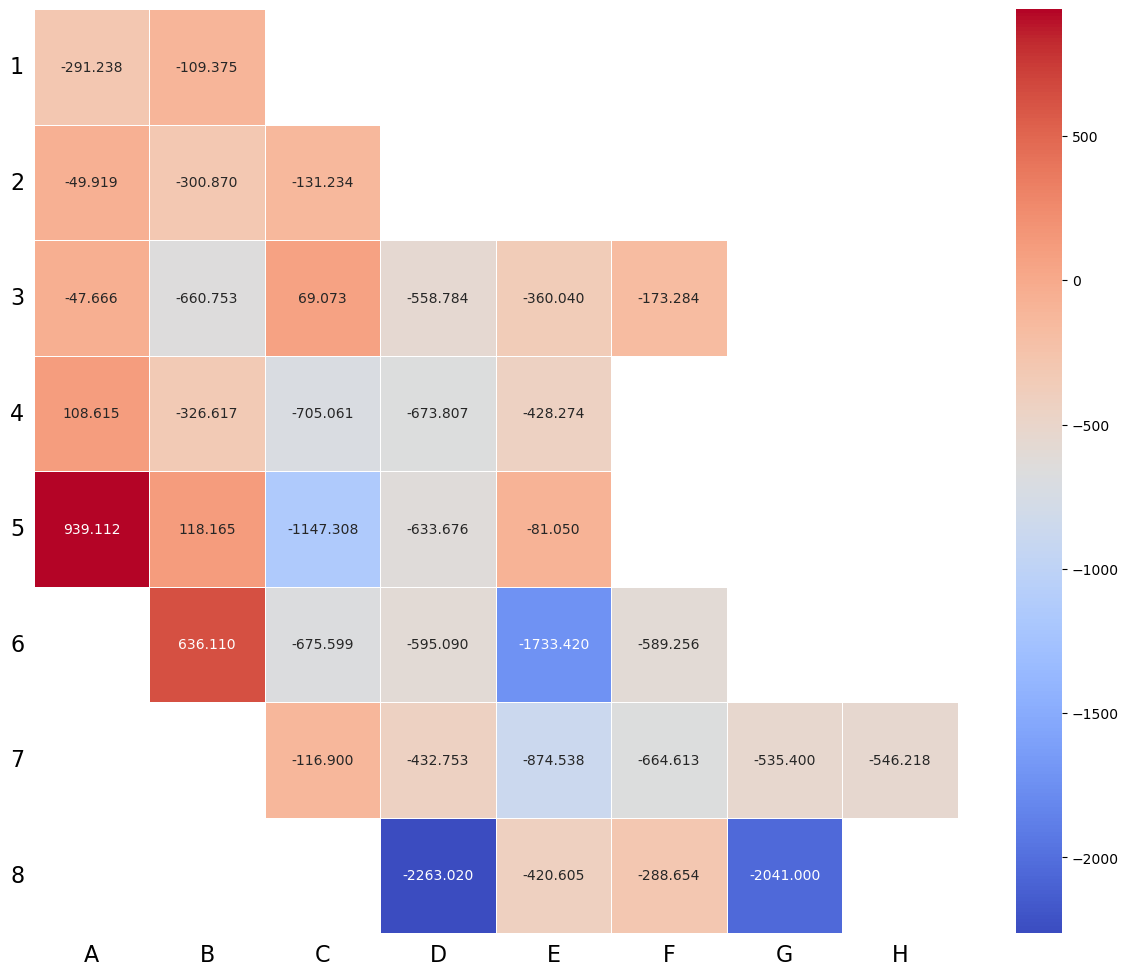
\includegraphics[trim={0 0 0 0},clip,scale=0.45]{Images/heatmap_pm25Anomaly250.png}
%}
%\caption{\bf PM$_{2.5}$ file Images/heatmap\_pm25Anomaly250.png}  
% \label{fig:Heatmap250PM}
%\end{figure}

\begin{figure}
\centering
%\fbox{
%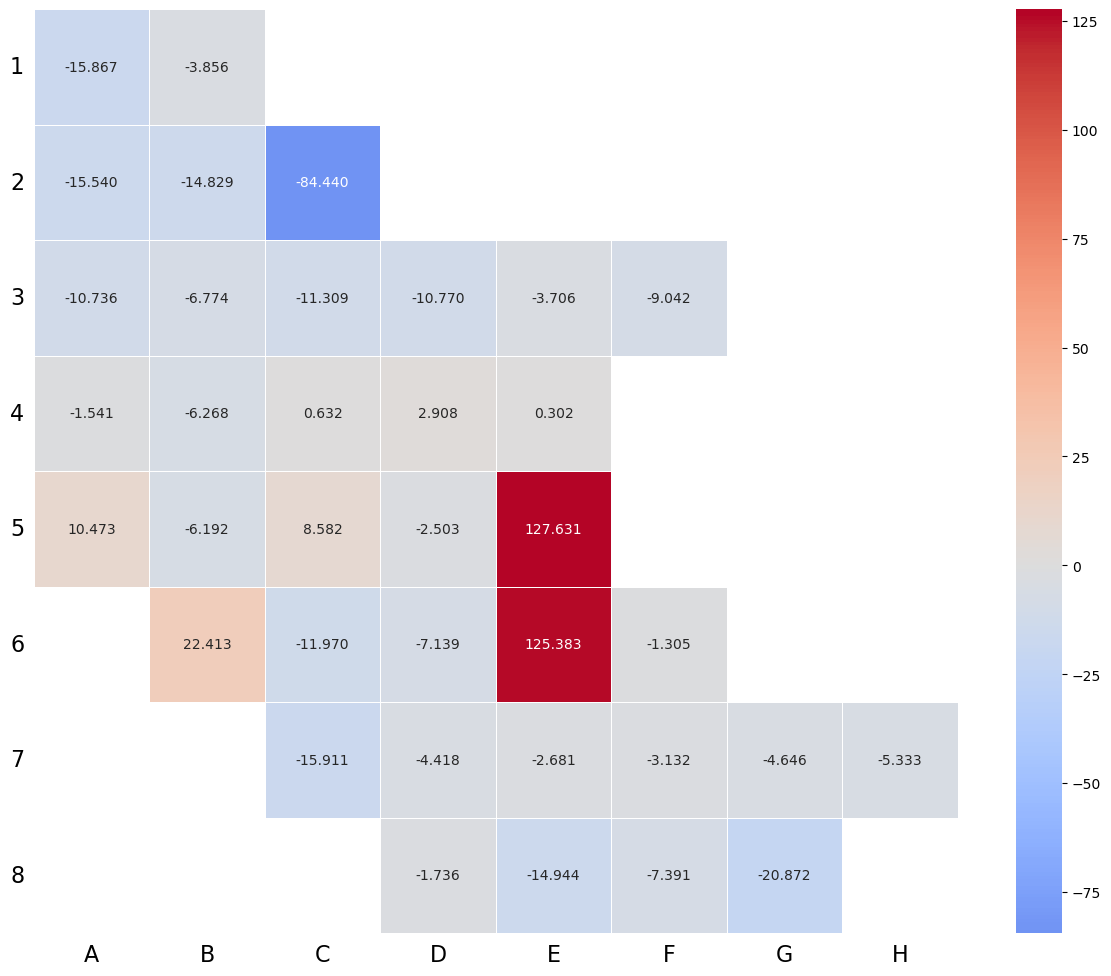
\includegraphics[trim={0 0 0 0},clip,scale=0.45]{Images/heatmap_no2Reduction7Ave7Ave250.png}

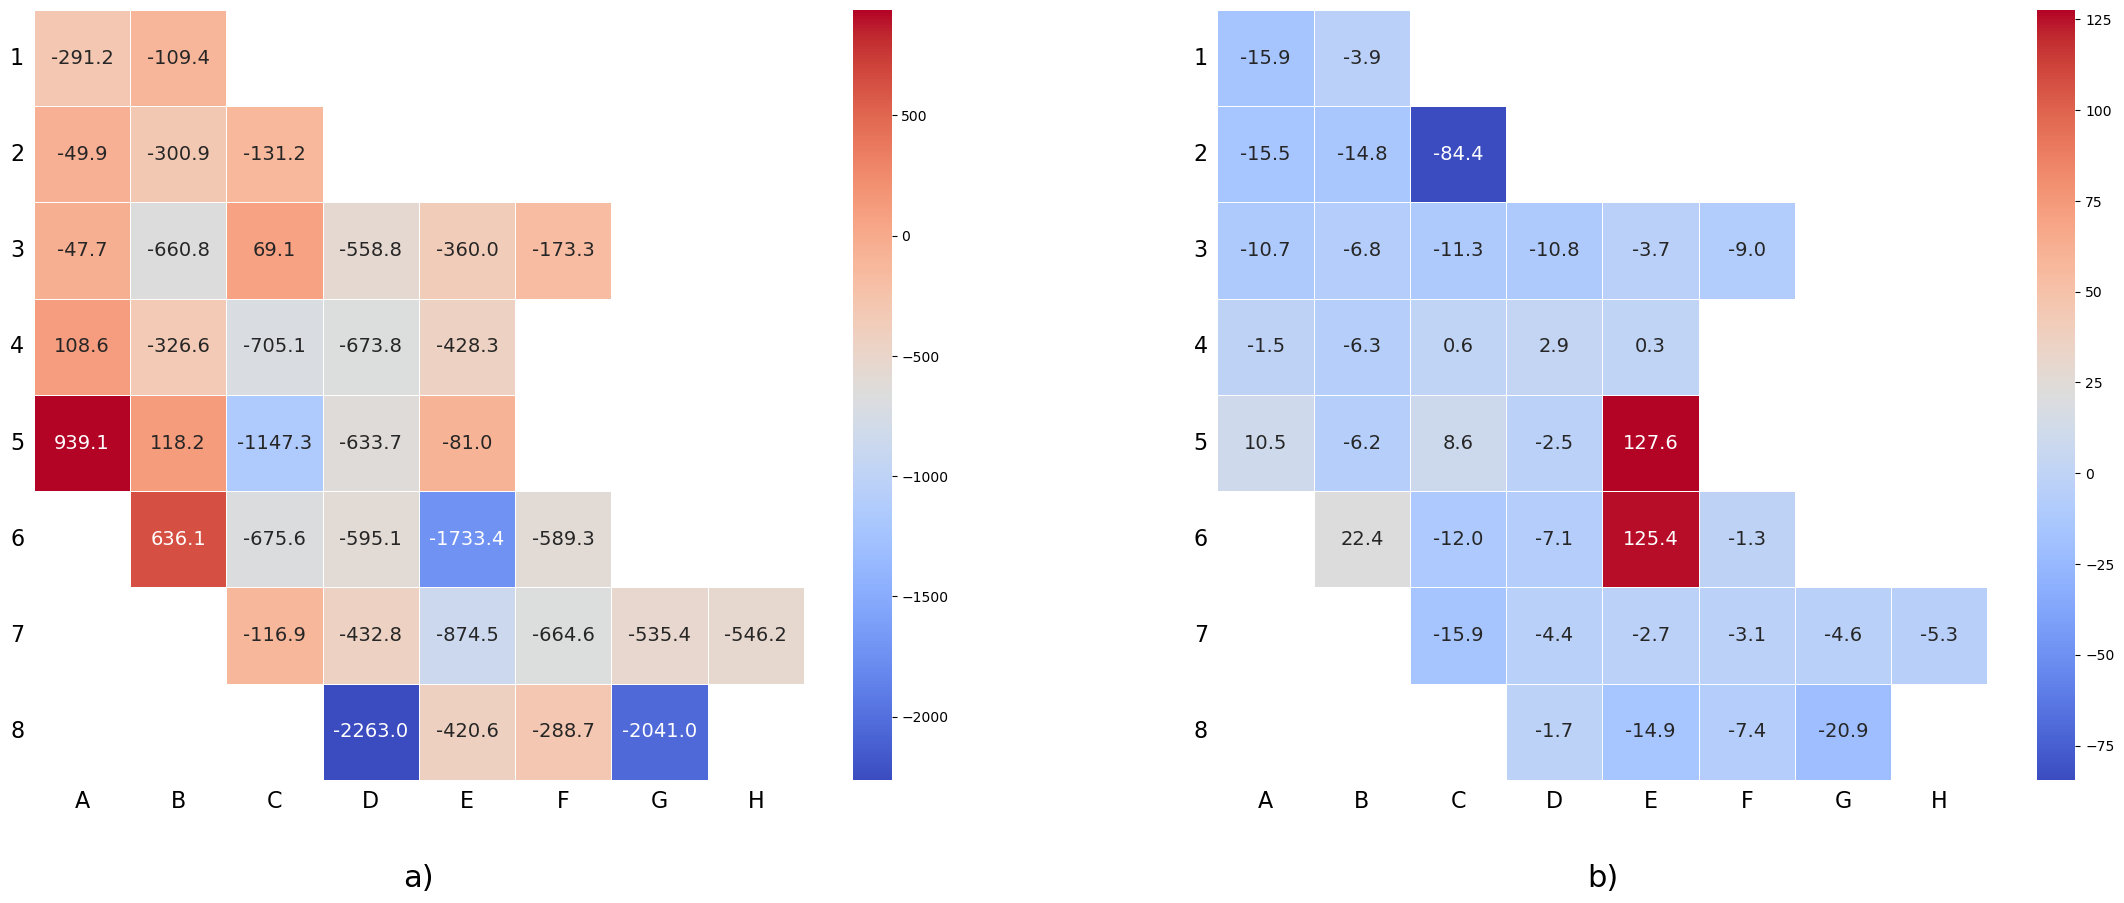
\includegraphics[trim={0 0 0 0},clip,scale=0.25]{Images/pm25Anomaly250_no2Reduction7Ave7Ave250.png}
%}
\caption{\bf Mean anomalies of a) PM$_{2.5}$ and b) NO$_{2}$ across the period of days 84 to 250 in 2020 for cities in each grid reference tile.}  
 \label{fig:Heatmap250NO2}\label{fig:Heatmap250PM}
\end{figure}

The characteristic design of cities designed to promote the egress of motor vehicles is that they have planned, regular block layouts (for instance, square or rectangular block patterns) and have blocks of medium-size in comparison to other global cities\cite{Thompson2020}. Such vehicle-centric city designs are predominantly found in countries including the United States, Australia, Canada, New Zealand, and Argentina which have seen rapid urban expansion in the late 19th and early 20th centuries. During the CoVID-19 pandemic's `Mid Crisis' and `Recovery' phases, cities optimised for private vehicle transport afforded citizens a choice between public transit and private vehicle use. Given the public's fear of potential infectious disease transmission on public transit\cite{fernando2023shaping}, citizens who had the option to avoid public transit in favour of private vehicles did so en-mass. In these cities, public transit ridership did not rebound in the observation period. 


\begin{figure}
     \centering
    % \begin{subfigure}[b]{0.9\textwidth}
        % \centering
       \scriptsize a)~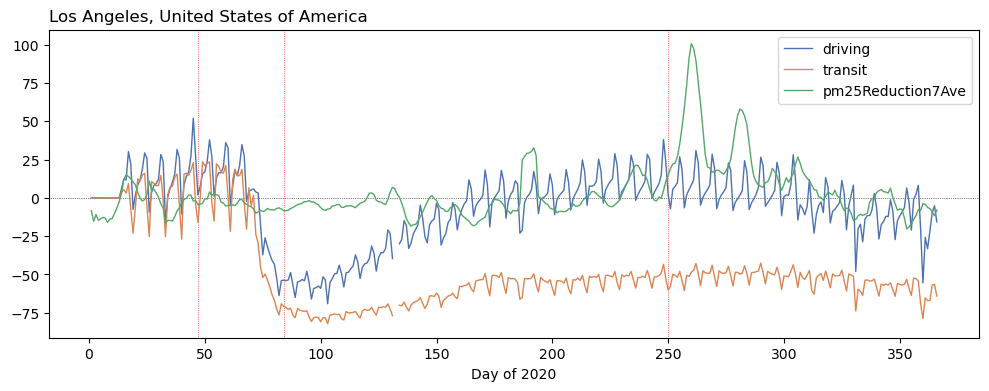
\includegraphics[width=\textwidth,trim={0 37 0 0},clip]{Images/LA_Drive_trans_pm25.png}
        % \caption{Los Angeles, United States of America}
         \label{fig:LosAngeles}
    % \end{subfigure}
     %\hfill
    % \begin{subfigure}[b]{0.9\textwidth}
       %  \centering
         b)~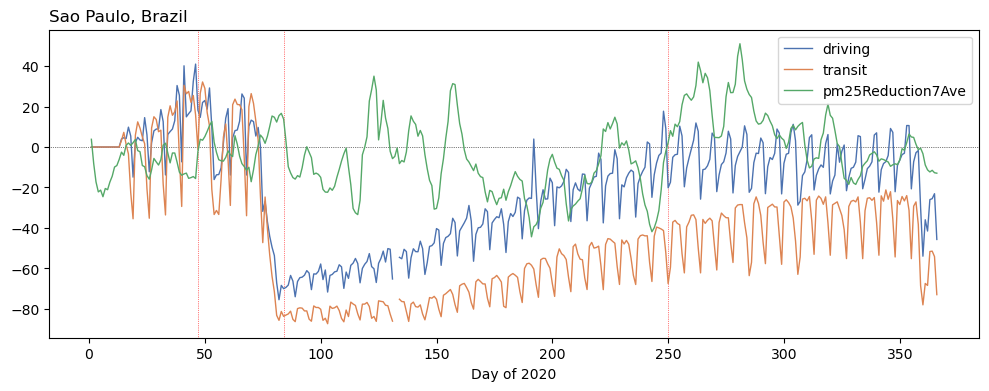
\includegraphics[width=\textwidth,trim={0 37 0 0},clip]{Images/SaoPaulo_Drive_trans_pm25.png}
         %\caption{Sao Paulo, Brazil}
         \label{fig:SaoPaulo}
    % \end{subfigure}
     %\hfill
    % \begin{subfigure}[b]{0.9\textwidth}
       %  \centering
         c)~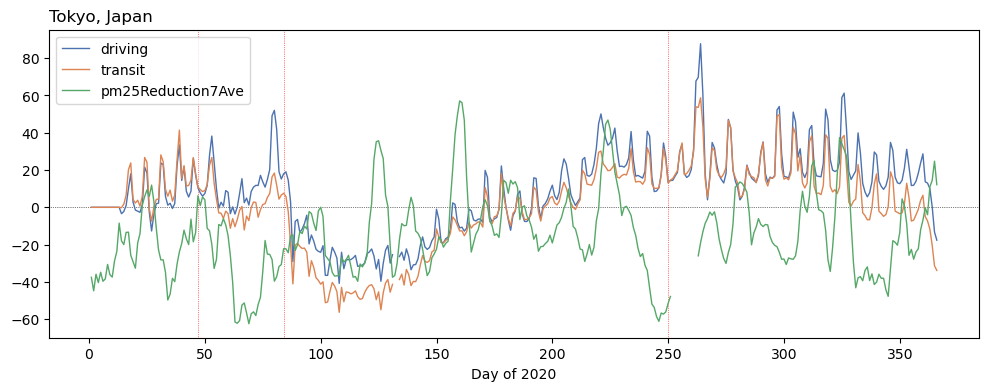
\includegraphics[width=\textwidth]{Images/Tokyo_Drive_trans_pm25.png}
        % \caption{Tokyo, Japan}
         \label{fig:Tokyo}
    % \end{subfigure}
        \caption{\bf An overview of the shifts in transportation mode preferences (daily Apple Mobility indexes for driving and transit modes in red and blue) and PM$_{2.5}$ anomalies over 2020 (7 day rolling averages of PM$_{2.5}$ anomalies in green) for a) Los Angeles, United States of America, b) S\~ao Paulo, Brazil and c) Tokyo, Japan. Highlighted is an increased reliance during the course of the CoVID-19 pandemic on private vehicle use over public transit in Los Angeles and S\~ao Paulo while minimal changes in transport mode share between public transit and private motor vehicles in Tokyo.}
        \label{fig:three_graphs_Driv_trans}
\end{figure}

For example, an archetypal city demonstrating a regular, car-based network is Los Angeles, USA. Figure \ref{fig:three_graphs_Driv_trans}a shows the relative change in mode share between public transit and private vehicles for Los Angeles from a pre-pandemic baseline during 2020 in addition to showing anomalies from expected levels of PM$_{2.5}$ pollution over the same period. Notable is that while observed patterns of mobility for Los Angeles' residents largely returned to normal in the second half of 2020, public transit ridership did not recover, but remained well below baseline. Importantly, the trade-off between public transit and private vehicle during the Recovery phase was also associated with a peak in PM$_{2.5}$ pollution. This pattern of results was observed across cities in North America and other cities located in grid areas A3 to A5 and B3 to B5 of Figure \ref{fig:tSNE} representing those with private car-based transport systems. In S\~ao Paulo, Brazil (Figure \ref{fig:three_graphs_Driv_trans}b), similar mobility shifts are seen. However, while Los Angeles transit rates stagnate at low levels across the remainder of 2020, transit usage in S\~ao Paulo begins to recover towards normal levels, although at a much slower rate than private vehicle use.

For the average of both North and South American locations, the combination of increased pollution levels, morbidity risk, and mobility dominated by private vehicle transport also coincided with the highest reported per-capita Covid-19 cases, globally (see Figure \ref{fig:covidCases7Ave}). 

\begin{figure}
\centering

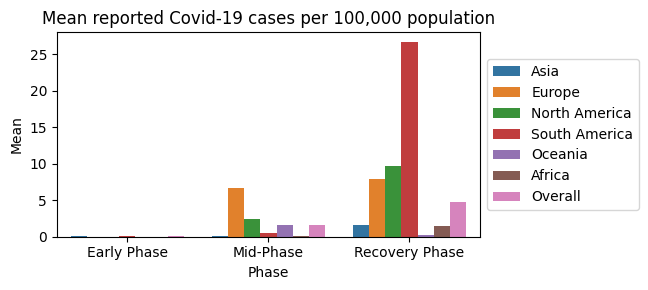
\includegraphics[trim={0 0 0 0},clip,scale=0.8]{Images/covidCases7Ave_plot.png}
%}
\caption{\bf Mean reported Covid-19 cases per 100,000 population across  continents in 2020 for the Early, Mid-Crisis, and Recovery pandemic phases.}  
 \label{fig:covidCases7Ave}\label{fig:Heatmap250PM}
\end{figure}

By contrast, Figure \ref{fig:three_graphs_Driv_trans}c demonstrates that the rebound in mobility in the second half of 2020 in the city of Tokyo, Japan did not result in a sustained modal shift between private vehicles and public transit. Similarly, neither did this rebound coincide with peaks in transport-related pollution nor widespread Covid-19 infection. This pattern of results was observed across Japanese cities, which are peculiar on the world stage in that they combine very dense road networks and very small blocks with high levels of public transit alongside policies that restrict on-street vehicle parking\cite{clements2019socialising}. This combination of city design and public policy shifts responsibility for parking provision onto individual vehicle owners rather than to local government, tipping the scales of transport choice away from private means and toward public and/or active transit. Therefore, while car-centric city designs afforded populations transport mode choice, Japanese cities and their supporting policies actively constrained citizens' options, resulting in a relative return to `normal' in the pandemic recovery phase.


\section*{Discussion}
The underlying structure and design of cities provides a basis upon which citizens move and interact. City designs can afford certain mode choices (e.g., driving or public transit) while constraining others (e.g., walking and cycling). Various patterns of movement and interaction facilitated by city designs translate into either direct (e.g., road crashes) or secondary risk exposures (e.g., exposure to airborne disease or pollution), that can then lead to injury and/or acute and chronic illness, increasing the global burden of disease.

The results presented here show that cities and populations across the world had different tools at their disposal in dealing with the threat posed by Covid-19, but their response to those threats also had both beneficial and harmful consequences at different phases of the crisis. This has lead some city types to demonstrate greater resilience than others.

First of all, there appears to have been a demonstrable reduction in pollution-related disease risk among most cities associated with mobility restrictions  enforced by governments seeking to reduce infection spread. Despite the threat posed by Covid-19 on an un-vaccinated population at the time, these secondary benefits were realised most acutely in the Entry and Mid-crisis phases of the pandemic when mobility was most greatly reduced; we estimate that risk of all-cause mortality and T2 Diabetes relative to a pre-pandemic baseline almost halved in many locations. Further, while no globally consistent data sources on road trauma at the city level are currently available, consistent evidence suggests that this period also saw a considerable reduction in road trauma across the world in both raw numbers of deaths and injuries \cite{saladie2023back} and also relative to other traumatic injuries (e.g., those incurred at home) \cite{WASEEM2021200}.

Unfortunately, many of these early benefits did not hold, even until the end of 2020. Further, with a desire to return to prior levels of mobility, many cities designed for private, car-based transport and where private vehicles have been preferenced over public or active transit options\cite{DAS20211}, appear to have already rebounded to levels of pollution and associated chronic disease risk that are equal to, if not exceeding, pre-pandemic levels. Added to this are post-pandemic rising rates of global road trauma associated with mode-shift away from  public transit ridership. Car-focused city designs across countries in North America, South America and Oceania appear to be contributing to even higher rates of road trauma than were experienced pre-pandemic \cite{ITFRS}. Meanwhile countries including Japan, South Korea, Norway, Sweden, and the Netherlands continue to enjoy steady declines in road trauma while maintaining high levels of mobility. 


More than half of the world's greenhouse gas (GHG) emissions have arisen in the period post the United Nations Framework Convention for Climate Change in 1992\cite{bashmakov2022climate}, with road transport one of the most significant contributors to these emissions. The societal challenge to mitigate GHG emissions by 2030 and net zero by 2050\cite{lynskey2020moving} is significant, highlighting the urgency to deliver pragmatic solutions now.

Japanese cities are peculiar on the world stage in that they combine a very dense road network with high levels of public transit and almost no on-street parking. This policy shifts responsibility for parking provision onto individual vehicle owners rather than to the public or local government. Therefore, while car-centric city designs afforded flexibility of choice to their populations, Japanese cities and supporting policies constrain citizens' options to easily shift between transportation modes.

The results above demonstrate that optimal city types for health are not static, but change given the health crises and concerns of the time. This should come as no surprise given the role of cities and shared urban infrastructure in historic public health disasters. However, the performance of cities and their role in producing or preventing disease has previously tended to be considered over a period of centuries, decades or years. Here, we demonstrate that optimal designs can also change in acute public health crises that unfold over weeks and months. City designs can facilitate rapid changes in mode-choice which may `stick' for better or worse. 

It therefore follows that the prestige and (ill-)health enjoyed by citizens in even the greatest or `healthiest' of cities or areas is perhaps ephemeral. Times, circumstances, environments, and conditions change that expose citizens to new risks and new public health challenges.


\section*{Conclusion}

\textbf{Funding} States the funding sources.

\section*{Contributors}\label{sec:credit}
KAN and JT conceived and designed the study and wrote the manuscript. KAN collected the data and analysed the data. HZ and SS performed data analysis and helped develop the methods. All authors contributed to writing and editing the manuscript.

\section*{Declaration of interests}\label{sec:dec}
We declare no competing interests.

\section*{Acknowledgments}\label{sec:ak}
KAN is supported by NHMRC/UKRI grant (1194959).





\bibliography{bibtext.bib}
\bibliographystyle{elsarticle-num} 
%\bibliography{bib}
\begin{thebibliography}{1}
\expandafter\ifx\csname url\endcsname\relax
  \def\url#1{\texttt{#1}}\fi
\expandafter\ifx\csname urlprefix\endcsname\relax\def\urlprefix{URL }\fi
\expandafter\ifx\csname href\endcsname\relax
  \def\href#1#2{#2} \def\path#1{#1}\fi

\end{thebibliography}


\section{Supplementary Material}
\beginsupplement

\begin{figure}
\centering
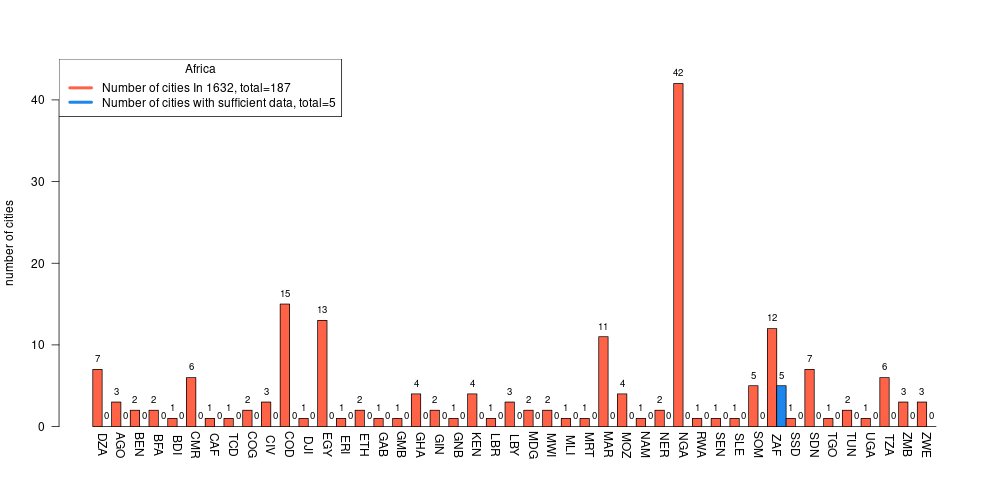
\includegraphics[trim={ 0 35 25 50 },clip,scale=0.45]{Images/Africa_cities.png}
\caption{\bf Number of the largest 1632 global cities in countries and the number of cities after excluding cities with insufficient data in Africa.}
 \label{fig:africa}
\end{figure}

\begin{figure}
\centering
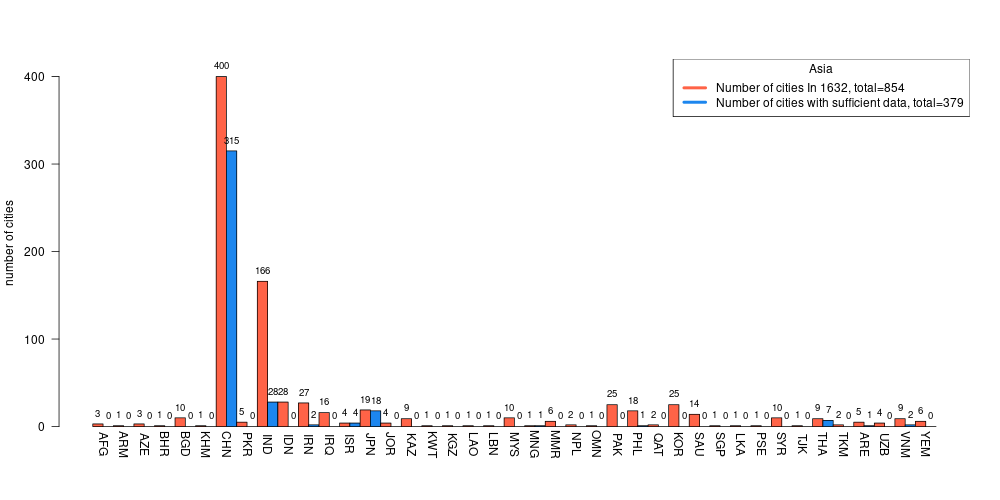
\includegraphics[trim={ 0 35 25 50 },clip,scale=0.45]{Images/Asia_cities.png}
\caption{\bf Number of the largest 1632 global cities in countries and the number of cities after excluding cities with insufficient data in Asia.}
 \label{fig:asia}
\end{figure}

\begin{figure}
\centering
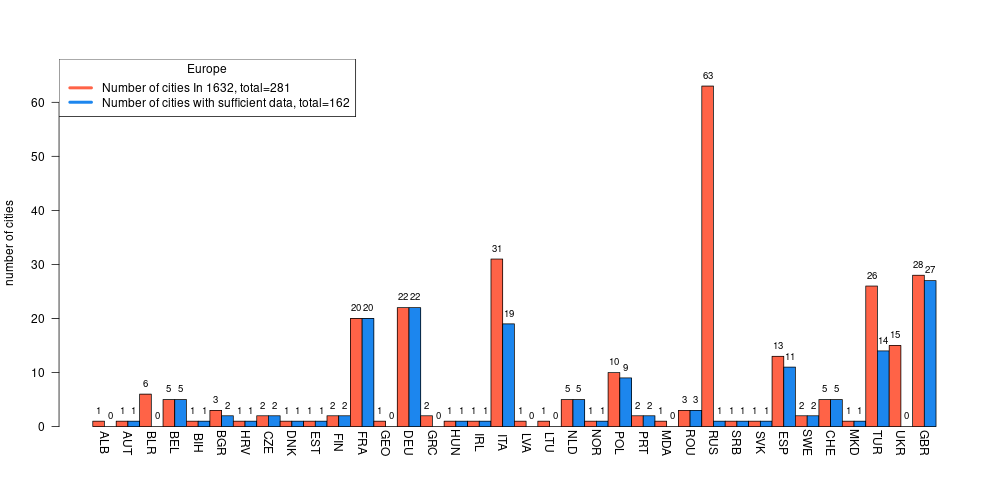
\includegraphics[trim={ 0 35 25 50 },clip,scale=0.45]{Images/Europe_cities.png}
\caption{\bf Number of the largest 1632 global cities in countries and the number of cities after excluding cities with insufficient data in Europe.}
 \label{fig:europe}
\end{figure}

\begin{figure}
\centering
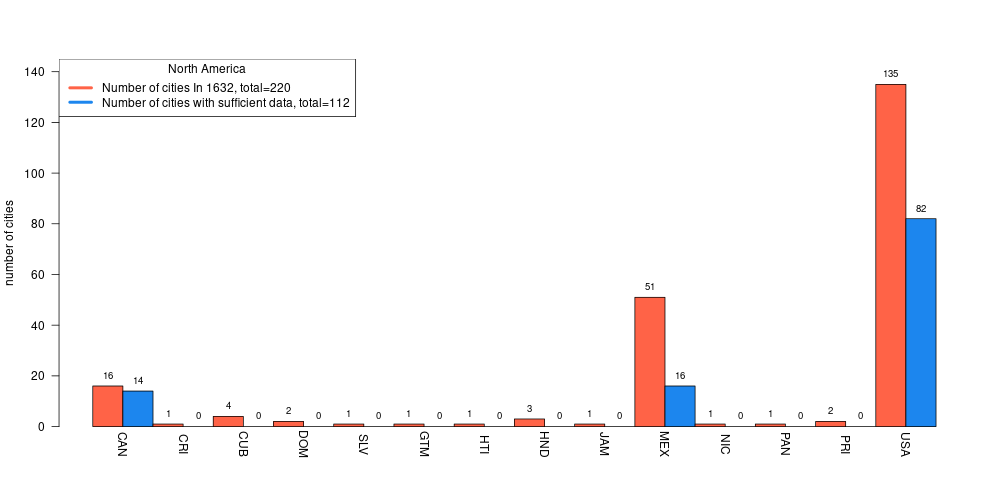
\includegraphics[trim={ 0 35 25 50 },clip,scale=0.45]{Images/North America_cities.png}
\caption{\bf Number of the largest 1632 global cities in countries and the number of cities after excluding cities with insufficient data in North America.}
 \label{fig:northamerica}
\end{figure}

\begin{figure}
\centering
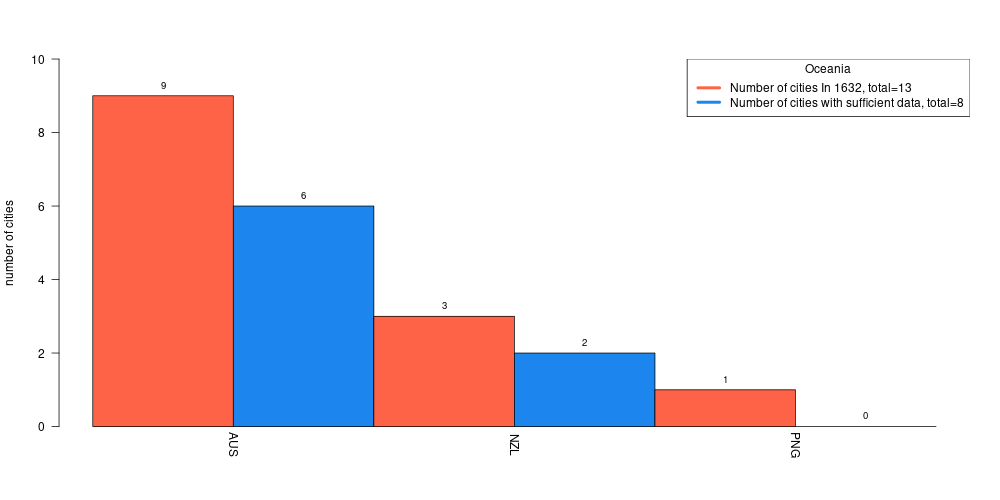
\includegraphics[trim={ 0 35 25 50 },clip,scale=0.45]{Images/Oceania_cities.png}
\caption{\bf Number of the largest 1632 global cities in countries and the number of cities after excluding cities with insufficient data in Oceania.}
 \label{fig:oceania}
\end{figure}

\begin{figure}
\centering
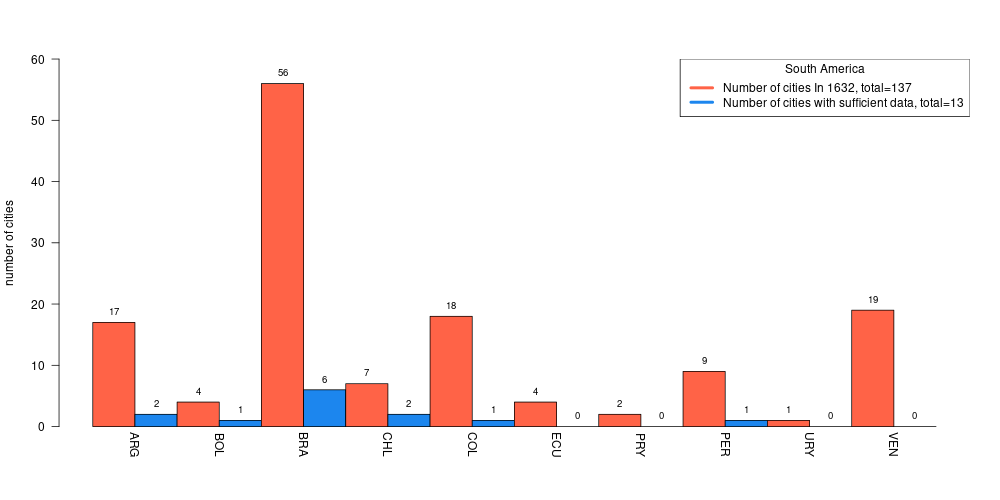
\includegraphics[trim={ 0 35 25 50 },clip,scale=0.45]{Images/South America_cities.png}
\caption{\bf Number of the largest 1632 global cities in countries and the number of cities after excluding cities with insufficient data in South America.}
 \label{fig:southhamerica}
\end{figure}


\end{document}
\endinput
%%
%% End of file `elsarticle-template-num.tex'.


